\chapter{Chapter 2: Linearized gravity and gravitational radiation\label{chp2}}
In this chapter we will introduce the concept of gravitational radiation in linearized gravity, which lead to the linearized gravitational field. A comparison of the radiation zone with electrodynamics is made. The main geometric contributions are calculated and a wave equation for gravitational radiation is obtained. A very important discussion of the nature of a background and a physical geometry is made, this became important for the energy contribution of the gravitational radiation. A energy-momentum tensor is obtained for the gravitational radiation, this allows to calculate the energy and momentum flux in terms of the linearized gravitational field. Finally an expression is obtained for the quadrupolar contribution of the gravitational radiation. Main references for this chapter are \cite{JACKSON,PAPER,CARROLL,THORNE-EX,MAGGIORE,GRAVITATION, HORTUA, POISSON, Isaacson-b, WinNT}

\section{Radiation zone}

Here we discuss the role of the radiation zone in gravitational radiation.
First we take a look of how the radiation zone is treated for far
away distances in electrodynamics and then we discuss its analogue
in gravitational radiation, which is the radiation zone in linearized
gravity.

\subsection{In Electrodynamics}

To describe the field of distributions from a certain distance of
a source, where the dimensions of the source are of order $d$, the
wavelength is $\lambda$ and $d\ll\lambda$, we split the space in
three spatial regions of interest
\[
\begin{array}{ll}
\text{The near (static) zone} & d\ll r\ll\lambda\\
\text{The intermediate (induction) zone} & d\ll r\sim\lambda\\
\text{The far (radiation) zone} & d\ll\lambda\ll r
\end{array}
\]

To study the fields in these regions we start from the Maxwell equations
\begin{align}
\nabla\cdot\boldsymbol{E}= & \ \frac{\rho}{\varepsilon_{0}}, & \nabla\cdot\boldsymbol{E}= & -\frac{\partial\boldsymbol{B}}{\partial t},\\
\nabla\cdot\boldsymbol{B}= & \ 0, & \nabla\cdot\boldsymbol{B}= & \ \mu_{0}\boldsymbol{J}+\mu_{0}\varepsilon_{0}\frac{\partial\boldsymbol{E}}{\partial t},
\end{align}
where $\boldsymbol{E}$ and $\boldsymbol{B}$ are the electric
and the magnetic field respectively, $\varepsilon_{0}$ is the vacuum
permittivity, $\mu_{0}$ is the vacuum permeability, $\rho$ in the
charge density and $\boldsymbol{J}$ is the current density. Now we
can arrive at the wave equations
\begin{align}
\left(\nabla^{2}-\frac{1}{c^{2}}\frac{\partial}{\partial t}\right)\boldsymbol{E}= & \ -\frac{1}{\varepsilon_{0}}\left(-\nabla\rho-\frac{1}{c^{2}}\frac{\partial\boldsymbol{J}}{\partial t}\right),\\
\left(\nabla^{2}-\frac{1}{c^{2}}\frac{\partial}{\partial t}\right)\boldsymbol{B}= & \ -\mu_{0}\nabla\times\boldsymbol{J}.
\end{align}
The solution to these equation is given by\footnote{See JACKSON, Section 6.4}
\begin{align}
\boldsymbol{E}\left(t,\boldsymbol{x}\right)= & \ \frac{1}{4\pi\varepsilon_{0}}\int\frac{1}{R}\left[-\nabla'\rho-\frac{1}{c^{2}}\frac{\partial\boldsymbol{J}}{\partial t'}\right]_{\text{ret}},\label{eq:elim}\\
\boldsymbol{B}\left(t,\boldsymbol{x}\right)= & \ \frac{\mu_{0}}{4\pi}\int\frac{1}{R}\left[\nabla'\times\boldsymbol{J}\right]_{\text{ret}},\label{eq:blim}
\end{align}
where $\left[\cdots\right]_{\text{ret}}$ means that the time $t'$
is to be evaluated at the retarded time $t'=t-\left|\boldsymbol{x}-\boldsymbol{x}'\right|/c$
and $R=\left|\boldsymbol{R}\right|=\left|\boldsymbol{x}-\boldsymbol{x}'\right|$.
In the equations (\ref{eq:elim}) and (\ref{eq:blim}), we can write
the static limits plus corrections
\begin{align}
\boldsymbol{E}\left(t,\boldsymbol{x}\right)= & \ \frac{1}{4\pi\varepsilon_{0}}\int\left\{ \frac{\hat{\boldsymbol{R}}}{R^{2}}\left[\rho\left(t',\boldsymbol{x}'\right)\right]_{\text{ret}}+\frac{\hat{\boldsymbol{R}}}{cR}\left[\frac{\partial\rho\left(t',\boldsymbol{x}'\right)}{\partial t'}\right]_{\text{ret}}\right.\nonumber \\
\  & \left.-\frac{\hat{\boldsymbol{R}}}{cR^{2}}\left[\frac{\partial\boldsymbol{J}\left(t',\boldsymbol{x}'\right)}{\partial t'}\right]_{\text{ret}}\right\} d^{3}x',\label{eq:egen}\\
\boldsymbol{B}\left(t,\boldsymbol{x}\right)= & \frac{\mu_{0}}{4\pi}\int\left\{ \left[\boldsymbol{J}\left(t',\boldsymbol{x}'\right)\right]_{\text{ret}}\times\frac{\hat{\boldsymbol{R}}}{R^{2}}+\left[\frac{\partial\boldsymbol{J}\left(t',\boldsymbol{x}'\right)}{\partial t'}\right]_{\text{ret}}\times\frac{\hat{\boldsymbol{R}}}{cR}\right\} d^{3}x',
\end{align}
where $\hat{\boldsymbol{R}}=\boldsymbol{R}/R$.

If the charge and current densities are time independent, the expressions
reduce to the static expressions
\begin{align*}
\boldsymbol{E}(\boldsymbol{x})= & \ \frac{1}{4\pi\varepsilon_{0}}\int\rho\left(\boldsymbol{x}'\right)\frac{\boldsymbol{x}-\boldsymbol{x}'}{\left|\boldsymbol{x}-\boldsymbol{x}'\right|}d^{3}x',\\
\boldsymbol{B}(\boldsymbol{x})= & \ \frac{\mu_{0}}{4\pi}\int\boldsymbol{J}\left(\boldsymbol{x}'\right)\times\frac{\boldsymbol{x}-\boldsymbol{x}'}{\left|\boldsymbol{x}-\boldsymbol{x}'\right|}d^{3}x'.
\end{align*}
In the case of the radiation fields, is better if we write the expression
(\ref{eq:egen}) just as follows
\begin{align*}
\boldsymbol{E}\left(t,\boldsymbol{x}\right)= & \ \frac{1}{4\pi\varepsilon_{0}}\int\left\{ \frac{\left[\rho\left(t',\boldsymbol{x}'\right)\right]_{\text{ret}}}{R^{2}}\hat{\boldsymbol{R}}+\frac{1}{cR^{2}}\left(\left[\boldsymbol{J}\left(t',\boldsymbol{x}'\right)\right]_{\text{ret}}\cdot\boldsymbol{R}\right)\boldsymbol{R}+\frac{1}{cR^{2}}\left(\left[\boldsymbol{J}\left(t',\boldsymbol{x}'\right)\right]_{\text{ret}}\times\boldsymbol{R}\right)\times\boldsymbol{R}\right.\\
\  & \ \left.\frac{1}{c^{2}R}\left(\left[\frac{\partial\boldsymbol{J}\left(t',\boldsymbol{x}'\right)}{\partial t'}\right]_{\text{ret}}\times\boldsymbol{R}\right)\times\boldsymbol{R}\right\} d^{3}x',
\end{align*}
in the radiation zone the term $1/R^{2}$ does not contribute to the
radiation field, then

\begin{align*}
\boldsymbol{E}(t,\boldsymbol{x})= & \ \frac{1}{4\pi\varepsilon_{0}}\int\frac{1}{c^{2}R}\left(\left[\frac{\partial\boldsymbol{J}\left(t',\boldsymbol{x}'\right)}{\partial t'}\right]_{\text{ret}}\times\boldsymbol{R}\right)\times\boldsymbol{R}d^{3}x',\\
\boldsymbol{B}(t,\boldsymbol{x})= & \ \frac{\mu_{0}}{4\pi}\int\frac{1}{cR}\left[\frac{\partial\boldsymbol{J}\left(t',\boldsymbol{x}'\right)}{\partial t'}\right]_{\text{ret}}\times\hat{\boldsymbol{R}}d^{3}x'.
\end{align*}
In the radiation zone we can write $\hat{\boldsymbol{R}}\approx\hat{\boldsymbol{x}}$,
$1/R\approx1/r$ and $R\approx r-\hat{\boldsymbol{x}}\cdot\boldsymbol{x}'$,
where $r=\left|\boldsymbol{x}\right|$, therefore we obtain

\begin{align*}
\boldsymbol{E}(t,\boldsymbol{x})\approx & \ \frac{1}{4\pi\varepsilon_{0}}\int\frac{1}{c^{2}R}\left(\left[\frac{\partial}{\partial t'}\boldsymbol{J}\left(t'+\frac{\hat{\boldsymbol{x}}\cdot\boldsymbol{x}'}{c},\boldsymbol{x}'\right)\right]\times\boldsymbol{R}\right)\times\boldsymbol{R}d^{3}x',\\
\boldsymbol{B}(t,\boldsymbol{x})\approx & \ \frac{\mu_{0}}{4\pi}\int\frac{1}{cR}\left[\frac{\partial}{\partial t'}\boldsymbol{J}\left(t'+\frac{\hat{\boldsymbol{x}}\cdot\boldsymbol{x}'}{c},\boldsymbol{x}'\right)\right]\times\hat{\boldsymbol{R}}d^{3}x',
\end{align*}
a comparison of aboves equations leads to
\[
\boldsymbol{E}\left(t,\boldsymbol{x}\right)=\boldsymbol{B}\left(t,\boldsymbol{x}\right)\times\hat{\boldsymbol{x}}.
\]

Given the charge conservation, the monopole contribution can not radiate,
but let us suppose that this can happend. If the monopole radiate
we will have a monopole term at a given time $t_{0}$
\[
\boldsymbol{E}_{m}=\frac{1}{4\pi\varepsilon_{0}c}\frac{\dot{Q}(t_{0})}{r}\hat{\boldsymbol{e}}_{r},
\]
where $\varepsilon_{0}$ is the vacuum permittivity. Then one could
thing that a sphere with an oscillating radius should radiate, but
according to Gauss's law, is exactly $(Q/4\pi\epsilon_{0}r^{2})\hat{\boldsymbol{r}}$,
regardless of the fluctiations in size. Therefore we find that the
radiation contributions starts from the dipole.

\subsection{In linearized gravity}

For the work of gravitational radiation we have to keep in mind, henceforth,
that gravitational waves propagates in a background curvature, notated
here by $\overline{g}_{\alpha\beta}(x)$. Under a suitable gauge,
we can split our metric tensor as follows
\begin{equation}
g_{\mu\nu}(x)=\overline{g}_{\alpha\beta}(x)+h_{\alpha\beta}(x),\label{eq:ggh}
\end{equation}
where the term $h_{\alpha\beta}$ is known as the \textbf{linearized
gravitational field}. Here we have not made any kind of aproximation
over $\overline{g}_{\alpha\beta}(x)$ neather $h_{\alpha\beta}(x)$
yet.

\begin{figure}[h]
\begin{centering}
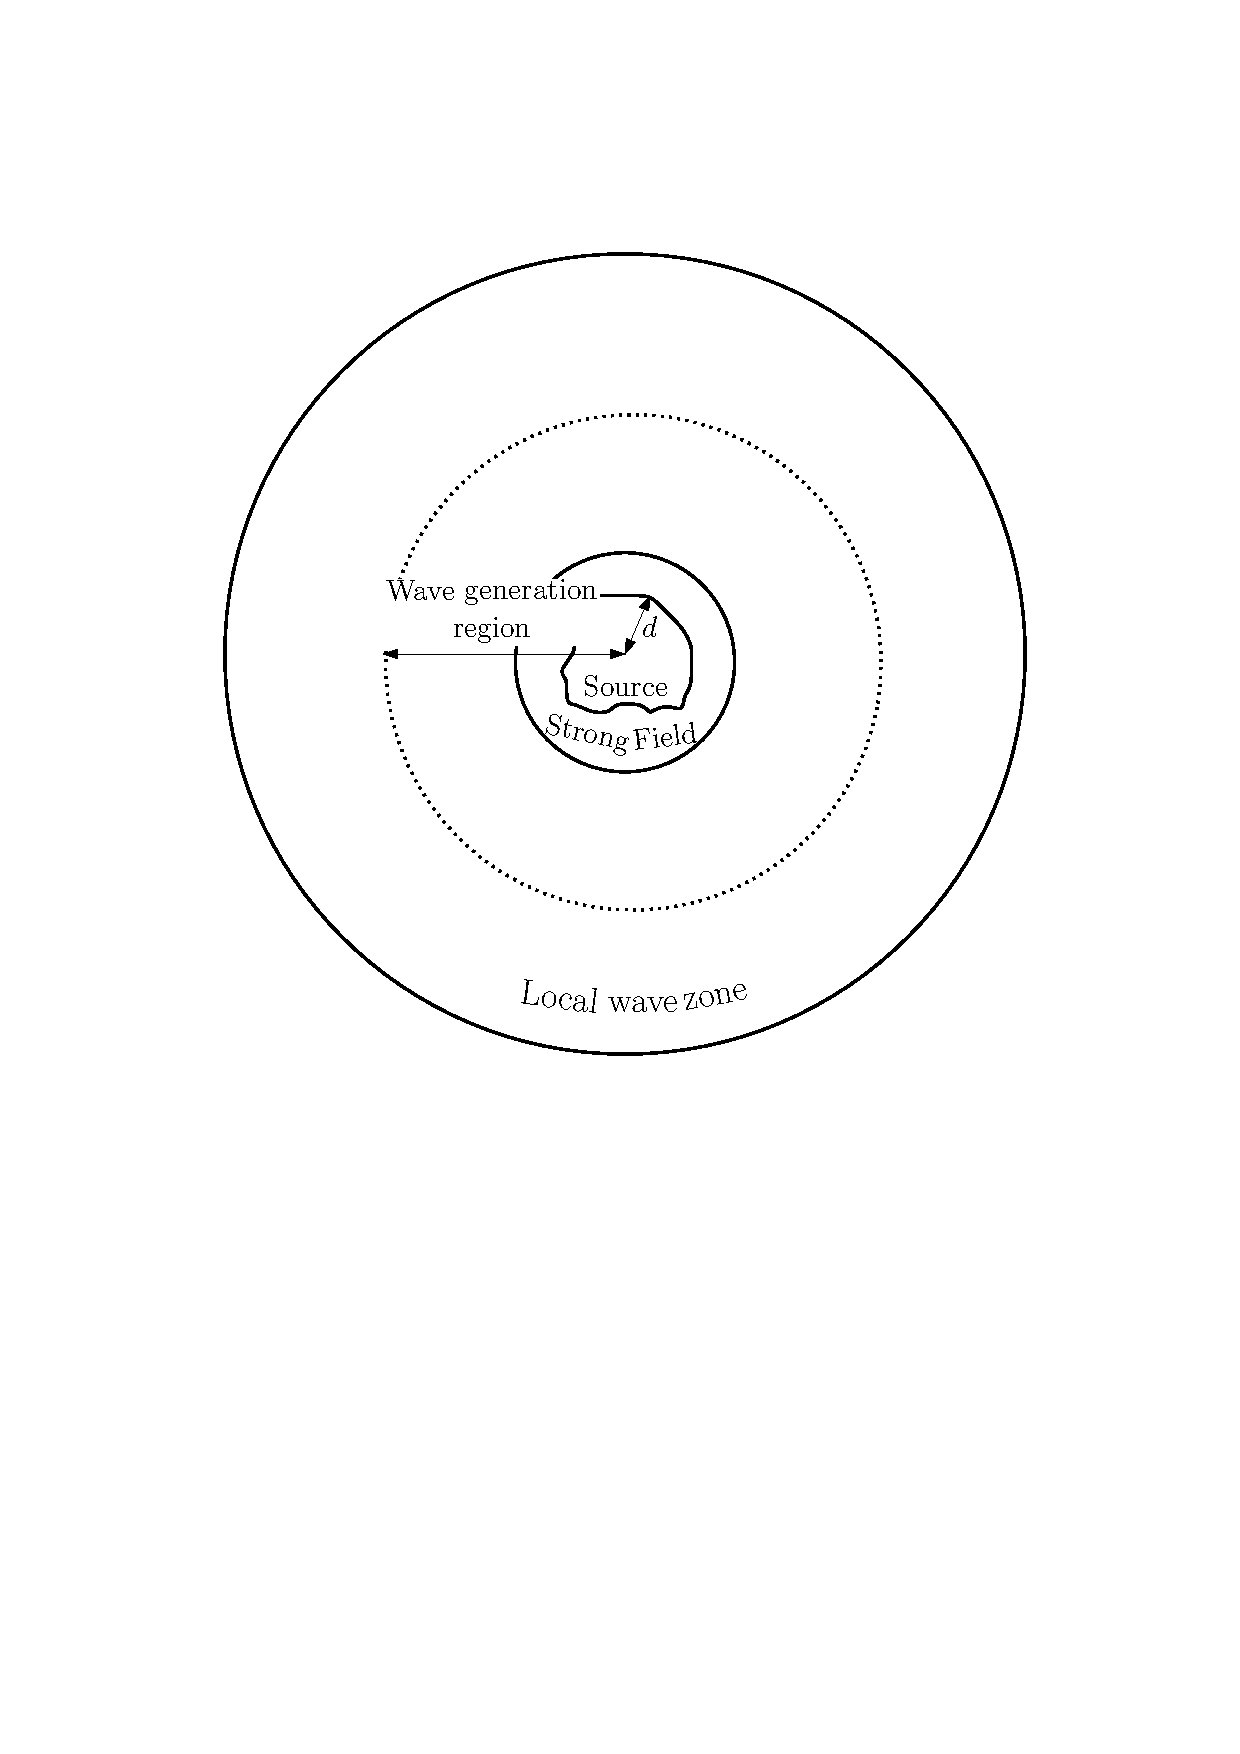
\includegraphics[scale=0.65]{Kap3/radiacion.pdf}\caption{Regions of spacetime surrounding a source. Traced image from \cite{THORNE-EX}. \label{figure1}}
\par\end{centering}
\end{figure}

For the case of linearized gravity, we are working in a region where
the source's waves are weak, so we can say that we have outgoing ripples
on a background spacetime where the effects of the background curvature
on the wave propagation are totally negligible. This region is called
the \textbf{local wave zone}, see figure \ref{figure1}, this region
is such that if $d$ is the size of the source, $\bar{\lambda}=\lambda/2\pi$
is the reduced wavelength of the gravitational wave and $r$ is the
radial coordinate of our system, then 
\[
d\ll\bar{\lambda}\ll r.
\]

This can be represented mathematically as
\begin{equation}
g_{\alpha\beta}=\eta_{\alpha\beta}+h_{\alpha\beta}\hspace{1em}\left|h_{\alpha\beta}\right|\ll1,\label{gl}
\end{equation}
where $\eta_{\alpha\beta}$ is the flat Minfkowski metric with
\[
\eta_{\alpha\beta}=\text{diag}\left(-1,1,1,1\right),
\]
then in the local wave zone the components of the metric only differ
slightly from the Minkowski form, then it will be adequate to treat
$h_{\alpha\beta}$ as a linearized field residing in flat spacetime.
Therefore $h^{\mu\nu}=\eta^{\mu\alpha}\eta^{\nu\beta}h_{\alpha\beta}$
and 
\[
g^{\alpha\beta}=\eta^{\alpha\beta}-h^{\alpha\beta}.
\]

\section{Gauge transformations in linearized gravity}

In this section we are going to deal with the gauge invariance issue.
This issue arises in the fact that we can use another coordinate system
where we can write $g_{\alpha\beta}$ just like in (\ref{gl}), but
with a totally different $h_{\alpha\beta}$, then we have a non unique
decomposition.

\begin{figure}[h]
\begin{centering}
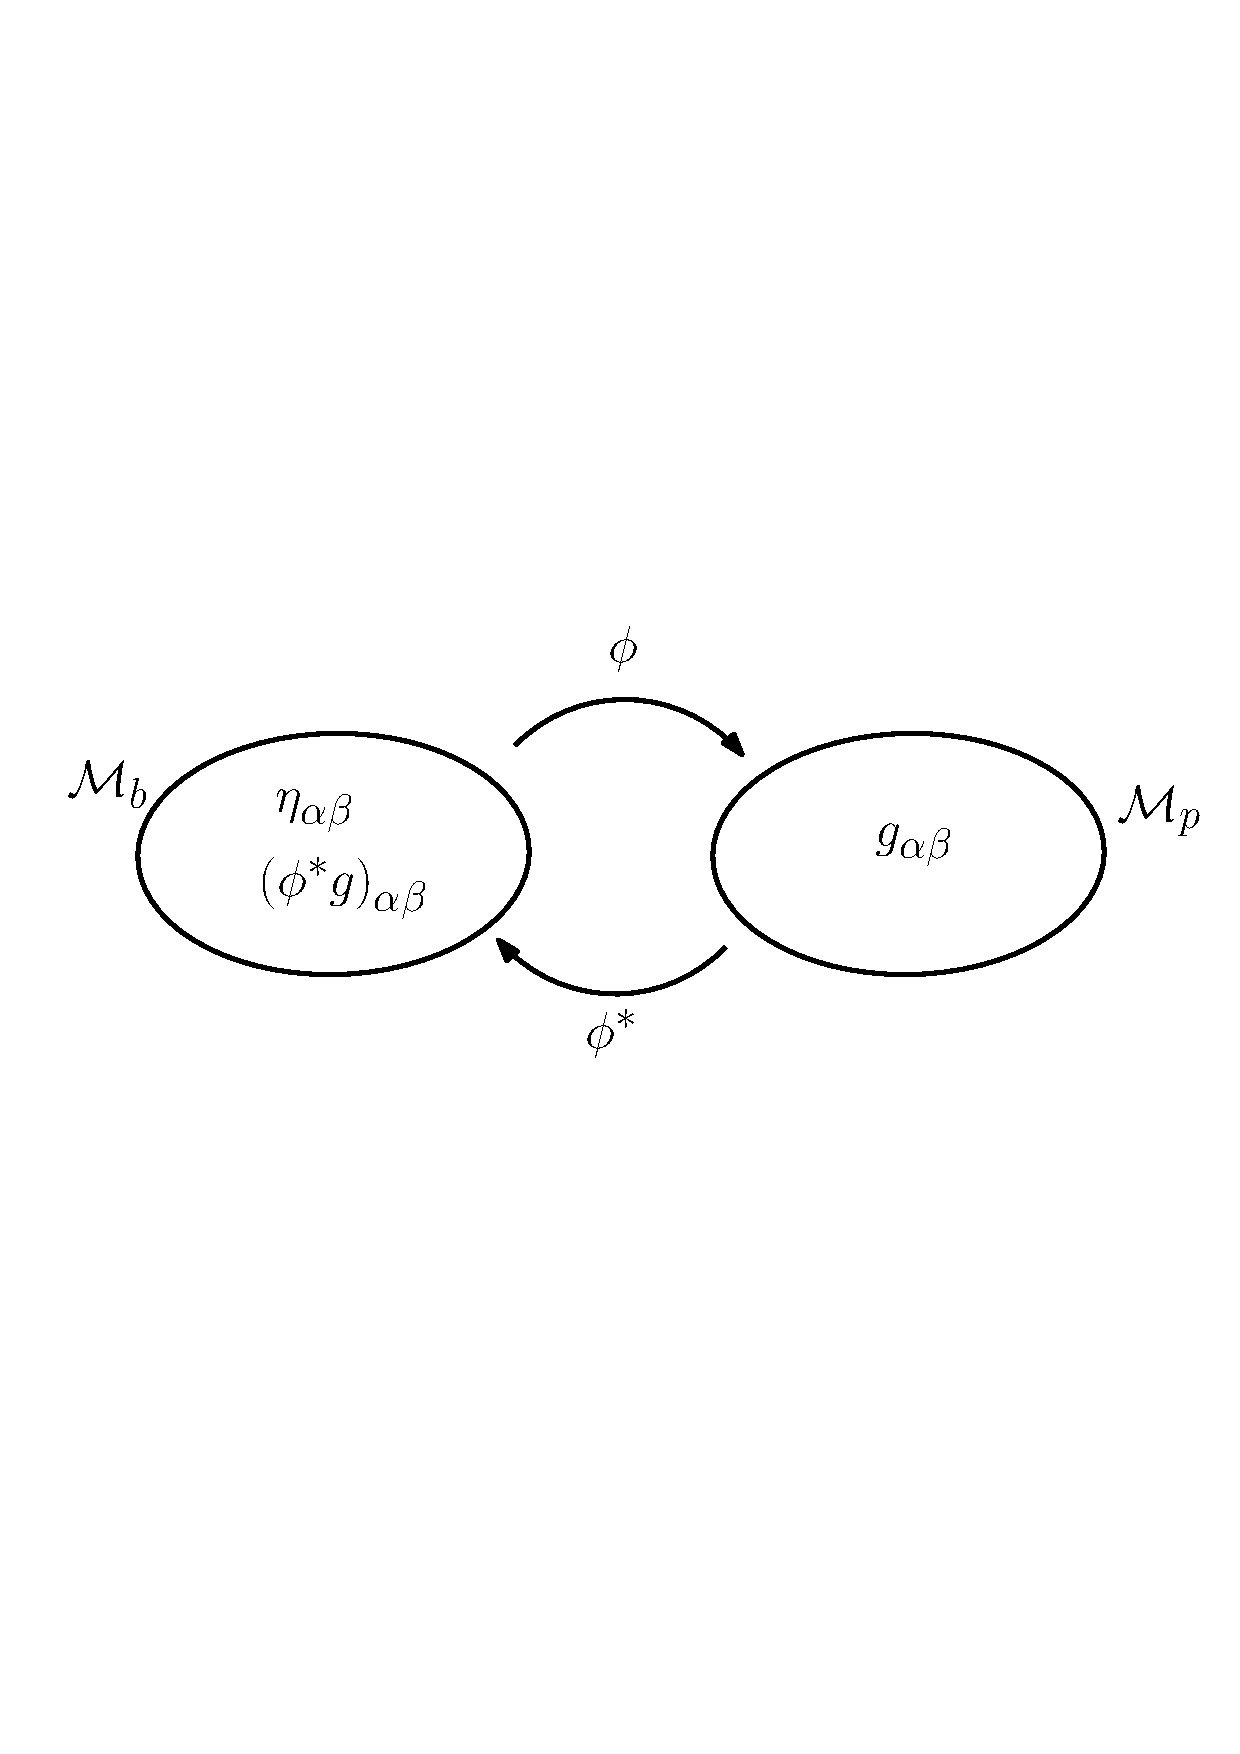
\includegraphics[scale=0.5]{Kap3/diffeof.pdf}\caption{A diffeomorphism relating the background spacetime $\mathcal{M}_{b}$,
with flat spacetime $\eta_{\alpha\beta}$, to the physical spacetime
$\mathcal{M}_{p}$. Traced image from \cite{CARROLL}. \label{fig:diff}}
\par\end{centering}
\end{figure}

We can formalize our concept of background in terms of a background
spacetime $\mathcal{M}_{b}$ , a physical spacetime $\mathcal{M}_{p}$
and a diffeomorphism between these manifolds, see figure \ref{fig:diff}
\[
\phi:\mathcal{M}_{b}\rightarrow\mathcal{M}_{p}.
\]
Because the diffeomorphism $\phi$, these manifolds describe the spacetime
in the same way: we are assigning events from the background spacetime
to the physic spacetime. In $\mathcal{M}_{b}$ we have defined the
flat Minkowski metric $\eta_{\alpha\beta}$, while in $\mathcal{M}_{p}$
we have defined some metric $g_{\alpha\beta}$ that obey's Einstein
field equations. Using the pullback function $\phi^{*}$ induced by
$\phi$, we have that $\left(\phi^{*}g\right)_{\alpha\beta}$ lives
in $\mathcal{M}_{b}$, then we define the linearized gravitational
field as
\begin{equation}
h_{\alpha\beta}=\left(\phi^{*}g\right)_{\alpha\beta}-\eta_{\alpha\beta}.\label{hd}
\end{equation}
From this definition, there is no reason for the components of $h_{\alpha\beta}$
to be small. However, because we are working in the local wave zone,
we limit our attention only to those diffeomorphisms for which $\left|h_{\alpha\beta}\right|\ll1$
is true. Through $\phi$, what we can said about $g_{\alpha\beta}$
and $h_{\alpha\beta}$ is that because $g_{\alpha\beta}$ obey's Einstein's
field equations on the physical spacetime, then $h_{\alpha\beta}$
will obey the linearized equation on the background spacetime.

\begin{figure}[h]
\centering{}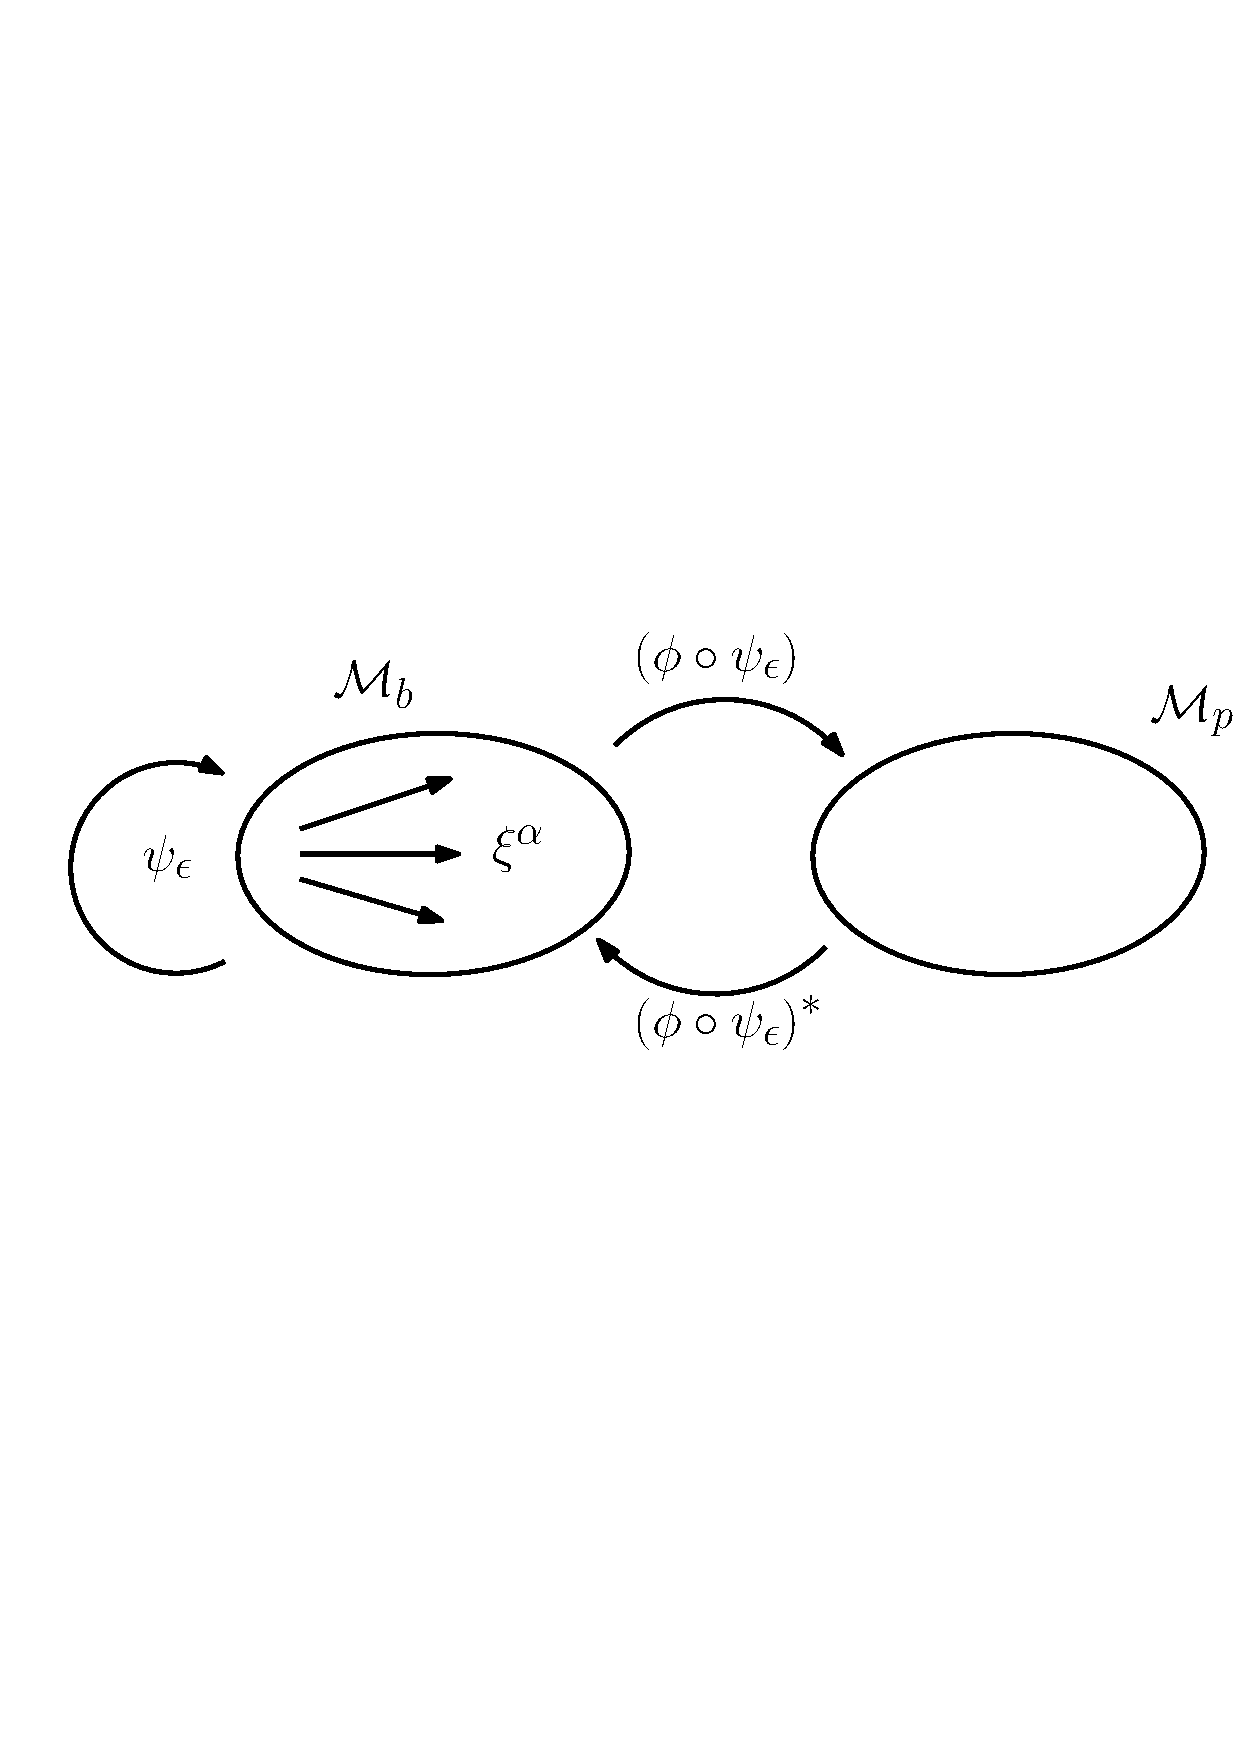
\includegraphics[scale=0.5]{Kap3/ediff.pdf}\caption{A one-parameter family of diffeomorphism $\psi_{\epsilon}$, generated
by the vector field $\xi^{\alpha}$ on the background spacetime $\mathcal{M}_{b}$.  Traced image from \cite{CARROLL}.\label{fig:ediff}}
\end{figure}

Now let us consider a vector field $\xi^{\alpha}(x)$ on $\mathcal{M}_{b}$.
This vector field generates a one-parameter family of diffeomorphism,
see figure \ref{fig:ediff},
\[
\psi_{\epsilon}:\mathcal{M}_{b}\rightarrow\mathcal{M}_{p}.
\]
For $\epsilon$ sufficiently small, if $\phi$ is a diffeomorphism for
which $h_{\alpha\beta}$ defined by (\ref{hd}) is small, then so
will $\left(\phi\circ\psi_{\epsilon}\right)$ be, but the perturbation
will have a different value. Then, we can define a family of perturbations
parametrized by $\epsilon$
\[
\begin{array}{ccl}
h_{\alpha\beta}^{(\epsilon)} & = & \left[\left(\phi\circ\psi_{\epsilon}\right)^{*}g\right]_{\alpha\beta}-\eta_{\alpha\beta}\\
\  & = & \left[\psi_{\epsilon}^{*}\left(\phi g\right)^{*}\right]_{\alpha\beta}-\eta_{\alpha\beta}\\
\  & = & \psi_{\epsilon}^{*}\left(h+\eta\right)_{\alpha\beta}-\eta_{\alpha\beta}\\
\  & = & \psi_{\epsilon}^{*}\left(h_{\alpha\beta}\right)+\psi_{\epsilon}^{*}\left(\eta_{\alpha\beta}\right)-\eta_{\alpha\beta}\\
\  & = & {\displaystyle \psi_{\epsilon}^{*}\left(h_{\alpha\beta}\right)+\epsilon\left(\frac{\psi_{\epsilon}^{*}\left(\eta_{\alpha\beta}\right)-\eta_{\alpha\beta}}{\epsilon}\right).}
\end{array}
\]
We use the fact that $\epsilon$ is small, then $\psi_{\epsilon}^{*}\left(h_{\alpha\beta}\right)=h_{\alpha\beta}$,
now using the definition of a Lie derivative
\[
h_{\alpha\beta}^{(\epsilon)}=h_{\alpha\beta}+\epsilon\mathcal{L}_{\xi}\eta_{\alpha\beta},
\]
from the fact that the background metric is flat
\begin{equation}
h_{\alpha\beta}^{(\epsilon)}=h_{\alpha\beta}+\epsilon\left(\partial_{\alpha}\xi_{\beta}+\partial_{\beta}\xi_{\alpha}\right).\label{he}
\end{equation}
This formula represents the change of the linearized gravitational
field under an infinitesimal diffeomorphism along the vector field
$\epsilon\xi^{\alpha}$. We will call this a \textbf{gauge transformation}
in linearized theory. The interpretation of the physical situations
through transformations is what is called active transformations,
for a deeper analysis of this see \cite{HORTUA}.

The diffeomorphism $\psi_{\epsilon}$ provide a different representation
of the same physical situation, while maintaining our requirement
that the linearized gravitational field is small. Then the result
(\ref{he}) tells us that the linearized gravitational fields that
denote physically equivalent spacetimes are related to each other
by $\epsilon\left(\partial_{\alpha}\xi_{\beta}+\partial_{\beta}\xi_{\alpha}\right)$
for some vector $\xi_{\alpha}$. This gauge invariance can also be
understood in the following way: the diffeomorphism $\psi_{\epsilon}$
can be thought of as the coordinate transformation
\begin{equation}
x^{\alpha}\rightarrow x^{\alpha}-\epsilon\xi^{\alpha},\label{ee}
\end{equation}
through the usual rules for transforming tensors under coordinate
transformations we can obtain the expression (\ref{he}). Typically
the value of $\epsilon$ is set to one and the vector field $\xi^{\alpha}$
itself as small.

\section{Linearized Einstein field equations}

In this section we will write the Einstein field equations in terms
of the linearized gravitational field, then we will see gravitational
contribution of $h_{\alpha\beta}$. It is important to remark that
here we are going to derivate with respect our background spacetime,
then we have to use the backgrounds spacetime covariant derivative,
which in this particular case is $\partial_{\text{\ensuremath{\alpha}}}$.

\subsection{General linearized expression of Einstein field equations}

From the expression (\ref{eq:chriss}) and (\ref{gl})
\[
\Gamma_{\beta\gamma}^{\alpha}=\frac{1}{2}\eta^{\alpha\sigma}\left(\partial_{\beta}h_{\gamma\sigma}+\partial_{\gamma}h_{\sigma\beta}-\partial_{\sigma}h_{\beta\gamma}\right).
\]
The contributions to the Riemann tensor will come only from the derivatives
of the $\Gamma$'s terms, then
\[
R_{\alpha\beta\gamma\delta}=\frac{1}{2}\left(\partial_{\gamma}\partial_{\beta}h_{\alpha\delta}+\partial_{\delta}\partial_{\alpha}h_{\beta\gamma}-\partial_{\delta}\partial_{\beta}h_{\alpha\gamma}-\partial_{\gamma}\partial_{\alpha}h_{\beta\delta}\right).
\]
Contracting over $\alpha$ and $\delta$ we obtain the Ricci tensor
\[
R_{\alpha\beta}=\frac{1}{2}\left(\partial_{\sigma}\partial_{\beta}h_{\alpha}^{\sigma}+\partial_{\sigma}\partial_{\alpha}h_{\beta}^{\sigma}-\partial_{\alpha}\partial_{\beta}h-\boxempty h_{\alpha\beta}\right),
\]
where $h=\eta^{\alpha\beta}h_{\alpha\beta}$ and $\boxempty=\eta^{\alpha\beta}\partial_{\alpha}\partial_{\beta}$,
the D'Alembert operator in flat spacetime. Contracting again we obtain
the Ricci scalar
\[
R=\partial_{\alpha}\partial_{\beta}h^{\alpha\beta}-\boxempty h,
\]
and with this we can obtain the Einstein tensor
\[
G_{\alpha\beta}=\frac{\text{1}}{2}\left(\partial_{\sigma}\partial_{\beta}h_{\alpha}^{\sigma}+\partial_{\sigma}\partial_{\alpha}h_{\beta}^{\sigma}-\partial_{\alpha}\partial_{\beta}h-\boxempty h_{\alpha\beta}-\eta_{\alpha\beta}\partial_{\mu}\partial_{\nu}h^{\mu\nu}+\eta_{\alpha\beta}\boxempty h\right),
\]
from which the Einstein field equations are written as
\begin{equation}
\partial_{\sigma}\partial_{\beta}h_{\alpha}^{\sigma}+\partial_{\sigma}\partial_{\alpha}h_{\beta}^{\sigma}-\partial_{\alpha}\partial_{\beta}h-\boxempty h_{\alpha\beta}-\eta_{\alpha\beta}\partial_{\mu}\partial_{\nu}h^{\mu\nu}+\eta_{\alpha\beta}\boxempty h=-\frac{16\pi G}{c^{4}}T_{\alpha\beta}.\label{efet}
\end{equation}

Because we are in the local wave zone we do not have any kind of local
sources, then $T_{\alpha\beta}=0$, therefore the equation (\ref{efet})
turns into
\[
\partial_{\sigma}\partial_{\beta}h_{\alpha}^{\sigma}+\partial_{\sigma}\partial_{\alpha}h_{\beta}^{\sigma}-\partial_{\alpha}\partial_{\beta}h-\boxempty h_{\alpha\beta}-\eta_{\alpha\beta}\partial_{\mu}\partial_{\nu}h^{\mu\nu}+\eta_{\alpha\beta}\boxempty h=0.
\]

\subsection{The DeDonder gauge in linearized gravity}

First we introduce the \textbf{trace-reversed gravitational field
}as\footnote{This is a particularization of the radiation field in the Relaxed
Einstein field equations that we will see in \ref{chp3}.}
\begin{equation}
\overline{h}_{\alpha\beta}=h_{\alpha\beta}-\frac{1}{2}\eta_{\alpha\beta}h,\label{hbar}
\end{equation}
we observe that $\bar{h}\equiv\eta^{\alpha\beta}\bar{h}_{\alpha\beta}=-h$.
With this gravitational field we can rewrite the equations (\ref{efet})
as
\begin{equation}
\boxempty\bar{h}_{\alpha\beta}+\eta_{\alpha\beta}\partial^{\rho}\partial^{\sigma}\bar{h}_{\rho\sigma}-\partial^{\rho}\partial_{\beta}\bar{h}_{\alpha\rho}-\partial^{\rho}\partial_{\alpha}\bar{h}_{\rho\beta}=-\frac{16\pi G}{c^{4}}T_{\alpha\beta}.\label{efeh}
\end{equation}

In the DeDonder gauge condition we set the coordinate system to fulfill
the wave equation in the background spacetime, in this case
\[
\boxempty x^{\alpha}=0
\]
where $\boxempty=\eta^{\alpha\beta}\partial_{\alpha}\partial_{\beta}$.
This condition can be written as follows\footnote{See Appendix \ref{appendix-harm}.}
\begin{equation}
\partial^{\beta}\overline{h}_{\alpha\beta}=0.\label{hg}
\end{equation}
With this the equation (\ref{efeh}) can be written as
\begin{equation}
\boxempty\bar{h}_{\alpha\beta}=-\frac{16\pi G}{c^{4}}T_{\alpha\beta},\label{efh}
\end{equation}
where, for consistency 
\[
\partial^{\beta}T_{\alpha\beta}=0.
\]
If we take $T_{\alpha\beta}=0$, in local wave zone region, then equation
(\ref{efh}) is
\[
\boxempty\bar{h}_{\alpha\beta}=0.
\]

Returning for a moment to the gauge transformation problem we can
get a gauge transformation expression, just like in equation (\ref{he}).
Using the equations (\ref{he}) and (\ref{hbar}) we have the gauge
transformation
\[
\bar{h}_{\alpha\beta}^{(\epsilon)}=\bar{h}_{\alpha\beta}-\epsilon\left(\partial_{\alpha}\xi_{\beta}+\partial_{\beta}\xi_{\alpha}-\eta_{\alpha\beta}\partial_{\sigma}\xi^{\sigma}\right).
\]
From (\ref{hg})
\[
\partial^{\beta}\bar{h}_{\alpha\beta}^{(\epsilon)}=\partial^{\beta}\bar{h}_{\alpha\beta}-\boxempty\xi_{\alpha},
\]
but we must set
\[
\partial^{\beta}\bar{h}_{\alpha\beta}^{(\epsilon)}=0.
\]
Let $f_{\alpha}(x)=\partial^{\beta}\bar{h}_{\alpha\beta}(x)$, therefore
the vector field $\xi_{\alpha}$ must fulfill that 
\[
\boxempty\xi_{\alpha}(x)=f_{\alpha}(x).
\]
Let us denote $G(x)$ the Green's function of the d'Alembert operator,
so that
\[
\boxempty_{x}G(x-y)=\delta^{4}(x-y),
\]
then the corresponding solution is
\[
\xi_{\alpha}=\int G(x-y)f_{\alpha}(y)d^{4}x.
\]
For the DeDonder gauge to hold, we set $\xi_{\alpha}=0$.

\subsection{The Transverse-Traceless gauge}

Here we are going to see the different contributions of $h_{\alpha\beta}$,
with this we mean the scalar, vector and tensor contribution of the
linearized gravitational field. This contributions comes from $h_{00}$,
$h_{0i}$ and $h_{ij}$, where $i,j=1,2,3$. Under a well-behaved
boundary conditions we can set
\begin{equation}
h^{0\mu}=0,\hspace{1em}h_{\mu}^{\mu}=0,\hspace{1em}\eta^{\sigma\nu}\partial_{\nu}h_{\mu\sigma}=0.\label{gtt}
\end{equation}
Therefore we have a tensor, and only spatial, contribution from $h_{\mu\nu}$.
This is known as the TT (Transverse-Traceless) gauge and will be noted
as $h_{\mu\nu}^{TT}$. The equation of motion is then
\begin{equation}
\boxempty h_{\alpha\beta}^{TT}=0\label{htto}
\end{equation}
and its solution is given by 
\begin{equation}
h_{\alpha\beta}^{TT}=A_{\alpha\beta}e^{ik_{\sigma}x^{\sigma}},\label{htt}
\end{equation}
where $A_{\alpha\beta}$ is a constant, symmetric two rank tensor
which is traceless and purely spatial
\[
\begin{array}{rl}
A_{0\alpha}=0 & ,\\
\eta^{\alpha\beta}A_{\alpha\beta}=0 & ,
\end{array}
\]
and $k_{\alpha}$ is the wave vector. Replacing the solution (\ref{htt})
in (\ref{htto}) we found that
\[
k_{\sigma}k^{\sigma}=0,
\]
then (\ref{htt}) is a solution to the linearized equations if the
wave vector is null, for hence the gravitational waves propagate at
speed of light. We still need to ensure that the solution is transverse,
from (\ref{gtt})
\begin{equation}
k_{\beta}A^{\beta\alpha}=0,\label{kc}
\end{equation}
we say then that the wave vector is orthogonal to $A^{\alpha\text{\ensuremath{\beta}}}$.

If we assume a particular direction of propagation, that is taking
$k^{\alpha}$ such that
\begin{equation}
k^{\alpha}=\left(\frac{\omega}{c},0,0,\frac{\omega}{c}\right),\label{eq:kz}
\end{equation}
from (\ref{kc}) and the fact that $A_{\alpha\beta}$ is purely spatial
\[
A_{3\beta}=0.
\]
Therefore for $A^{\alpha\text{\ensuremath{\beta}}}$ we have the components
\[
A_{\alpha\beta}=\left(\begin{array}{cccc}
0 & 0 & 0 & 0\\
0 & A_{11} & A_{12} & 0\\
0 & A_{12} & -A_{11} & 0\\
0 & 0 & 0 & 0
\end{array}\right),
\]
these non-zero components characterize completely the linearized field
in this case. For these amplitudes following notation is used: $A_{11}=h_{+}$
and $A_{12}=h_{\times}$, then
\begin{equation}
A_{\alpha\beta}=\left(\begin{array}{cccc}
0 & 0 & 0 & 0\\
0 & h_{+} & h_{\times} & 0\\
0 & h_{\times} & -h_{+} & 0\\
0 & 0 & 0 & 0
\end{array}\right).\label{eq:A-plus-cross}
\end{equation}
These are called the ``plus'', $h_{+}$, and the ``cross'', $h_{\times}$,
polarizations of the wave. 

Now we are going to define a tensor that will allow us to find the
form of the wave in the TT gauge. First we introduce the tensor
\[
P_{ij}\left(\hat{\boldsymbol{n}}\right)=\delta_{ij}-n_{i}n_{j},
\]
where $\hat{\boldsymbol{n}}$ is $h_{\alpha\beta}$ propagating direction.
With this tensor we construct
\[
\Lambda_{ij,kl}\left(\hat{\boldsymbol{n}}\right)=P_{ik}P_{jl}-\frac{1}{2}P_{ij}P_{kl},
\]
this tensor is a projector, this means that
\[
\Lambda_{ij,kl}\Lambda_{kl,mn}=\Lambda_{ij,mn}.
\]
Furthermore, it is transverse on all its indices
\[
n^{i}\Lambda_{ij,kl}=n^{j}\Lambda_{ij,kl}=n^{k}\Lambda_{ij,kl}=n^{l}\Lambda_{ij,kl}=0,
\]
it is traceless with respect to the $\left(i,j\right)$ and $\left(k,l\right)$
indices
\[
\Lambda_{ii,kl}=\Lambda_{ij,kk}=0,
\]
and is symmetric under the simultaneous exchange $\left(i,j\right)\longleftrightarrow\left(k,l\right)$.
In terms of $\hat{\boldsymbol{n}}$, its explicit form is
\begin{align*}
\Lambda_{ij,kl} & =\delta_{ik}\delta_{jl}-\frac{1}{2}\delta_{ij}\delta_{kl}-n_{j}n_{l}\delta_{ik}-n_{i}n_{k}\delta_{jl}\\
\  & +\frac{1}{2}n_{k}n_{l}\delta_{ij}+\frac{1}{2}n_{i}n_{j}\delta_{kl}+\frac{1}{2}n_{i}n_{j}n_{k}n_{l}.
\end{align*}
The gravitational wave in the TT gauge is given in terms of the spatial
components $h_{ij}$ of $h_{\alpha\beta}$ by
\[
h_{ij}^{TT}=\Lambda_{ij,kl}h_{kl}
\]

For the study of the interaction of gravitational waves in linearized
gravity with test masses, see \cite{MAGGIORE}.

\subsubsection{Solution to the linearized equation}

Here we start from the equation (\ref{efh}), this can be solved by
the method of Green's function: if $G(\boldsymbol{x}-\boldsymbol{x}')$
is a solution of the equation
\begin{equation}
\boxempty_{\boldsymbol{x}}G\left(\boldsymbol{x}-\boldsymbol{x}'\right)=\delta^{4}\left(\boldsymbol{x}-\boldsymbol{x}'\right),\label{eq:green}
\end{equation}
where $\boxempty_{\boldsymbol{x}}$ is the d'Alembertian operator
with derivatives taken with respect to the variable $\boldsymbol{x}$,
then the corresponding solution of equation (\ref{efh}) is 
\[
\bar{h}_{\alpha\beta}=-\frac{16\pi G}{c^{4}}\int G\left(\boldsymbol{x}-\boldsymbol{x}'\right)T_{\alpha\beta}\left(\boldsymbol{x}'\right)d^{4}\boldsymbol{x}'.
\]

The solution of equation (\ref{eq:green}) depends of the boundary
conditions. Just as in electromagnetism, for a radiation problem the
appropriate solution is the retarded Green's function\footnote{For details see Box 6.5 from \cite{POISSON}}
\[
G\left(\boldsymbol{x}-\boldsymbol{x}'\right)=-\frac{1}{4\pi\left|\boldsymbol{x}-\boldsymbol{x}'\right|}\delta\left(x_{\text{ret}}^{0}-{x'}^{0}\right),
\]
where ${x'}^{0}=ct'$, $x_{\text{ret}}^{0}=ct_{\text{ret}}$ and 
\[
t_{\text{ret}}=t-\frac{\left|\boldsymbol{x}-\boldsymbol{x}'\right|}{c}
\]
is called retarded time. Then the solution of equation (\ref{efh})
is
\[
\bar{h}_{\alpha\beta}=\frac{4G}{c^{4}}\int\frac{1}{\left|\boldsymbol{x}-\boldsymbol{x}'\right|}T_{\alpha\beta}\left(t-\frac{\left|\boldsymbol{x}-\boldsymbol{x}'\right|}{c},\boldsymbol{x}'\right).
\]
Outside the source we can put this solution in the TT gauge using
the $\Lambda_{ij,kl}$ tensor

\[
h_{ij}^{TT}=\Lambda_{ij,kl}\bar{h}_{kl},
\]
therefore outside the source
\[
h_{ij}^{TT}=\frac{4G}{c^{4}}\Lambda_{ij,kl}\left(\hat{\boldsymbol{n}}\right)\int\frac{1}{\left|\boldsymbol{x}-\boldsymbol{x}'\right|}T_{\alpha\beta}\left(t-\frac{\left|\boldsymbol{x}-\boldsymbol{x}'\right|}{c},\boldsymbol{x}'\right).
\]

\subsection{Energy of gravitational waves in linearized gravity}

\subsubsection{The non-location of energy of the gravitational field}

In spite of there exist a mathematical tool to work with the energy
of the gravitational field\footnote{See section \ref{sec:energy}},
there is not such thing as a local gravity energy-momentum. It does
not curve the spacetime or serve as a source term on the Einstein's
field equations.

One can always find in any given locality a frame of reference in
which all Christoffel symbols disappear, but this does not mean that
there is no curvature. No $\Gamma$'s means no local gravitational
field and no local gravitational field means no local gravitational
energy momentum. We want to describe this now in a more mathematical
way, then we are going to introduce one example of a coordinate system
in which $\Gamma$'s are zero, this is the Riemann normal coordinates.
We pick an event $\mathcal{P}_{0}$ and a set of basis vectors $\left\{ \boldsymbol{e}_{\alpha}\left(\mathcal{P}_{0}\right)\right\} $
such that we have the following properties
\begin{align}
\boldsymbol{e}_{\alpha}\left(\mathcal{P}_{0}\right)=\  & {\displaystyle \left(\frac{\partial}{\partial x^{\alpha}}\right)_{\mathcal{P}_{0}}}\\
\Gamma_{\beta\gamma}^{\alpha}\left(\mathcal{P}_{0}\right)=\  & 0\\
\partial_{\mu}\Gamma_{\beta\gamma}^{\alpha}\left(\mathcal{P}_{0}\right)=\  & {\displaystyle -\frac{1}{3}\left(R_{\beta\gamma\mu}^{\alpha}+R_{\gamma\beta\mu}^{\alpha}\right)}.\label{eq:dgamma}
\end{align}

Then, just like is shown in equation (\ref{eq:dgamma}), the fact
that the $\Gamma$'s are zero does not mean that there is no curvature.

\subsubsection{Separation of gravitational radiation and background}

Here we take again the form of our metric tensor just like in equation
(\ref{eq:ggh}) but with the following condition: $\left|h_{\alpha\beta}\right|\ll1$.
The idea of this subsection is to discuss how to decide which part
of $g_{\alpha\beta}$ is a contribution given by $\overline{g}_{\alpha\beta}$
or by $h_{\alpha\beta}$. Just like the splitting between the spacetime
background and the linearized gravitational field, we can make a separation
of scales. We begging considering an exact plane-wave solution to
the Einstein field equations, this will allow us to compare the magnitude
of the values when we make the separation of scales. With this separation
of scales we can determine the scale contribution of $h_{\alpha\beta}$.

\subsubsection*{An exact plane-wave solution}

We are going to consider an exact solution of a plane wave first,
this to understand how the background curvature and the gravitational
radiation curvature can be distinguished. The solution that we are
going to consider is 
\begin{align*}
ds^{2}= & \ L^{2}\left(e^{2\beta}dx^{2}+e^{-2\beta}dy^{2}\right)+dz^{2}-c^{2}dt^{2}\\
= & \ L^{2}\left(e^{2\beta}dx^{2}+e^{-2\beta}dy^{2}\right)-dudv,
\end{align*}
where
\[
u=ct-z,\ v=ct+z,\ L=L\left(u\right),\ \beta=\beta\left(u\right).
\]
The function $L$ is known as the background factor and $\beta$ the
wave factor.

First we are going to calculate the non-vanishing components of the
Riemann tensor, for this we are going to use the variational principle.
Let us consider the equation
\begin{align*}
S & =\frac{1}{2}\int g_{\alpha\beta}\dot{x}^{\alpha}\dot{x}^{\beta}d\lambda\\
\  & =\int\left[\frac{1}{2}L^{2}\left(e^{2\beta}\dot{x}^{2}+e^{-2\beta}\dot{y}^{2}\right)-\dot{u}\dot{v}\right]d\lambda
\end{align*}
where $\dot{x}=dx/d\lambda$ where $\lambda$ is a parameter along
a curve. First vary $x\left(\lambda\right)$ keeping fixed the functions
$y\left(\lambda\right)$, $u\left(\lambda\right)$ and $v\left(\lambda\right)$
\begin{align*}
\delta S & =\int\left(L^{2}e^{2\beta}\dot{x}\right)\delta\dot{x}d\lambda=\int\left(L^{2}e^{2\beta}\dot{x}\right)^{\cdot}\delta xd\lambda=0,
\end{align*}
then
\[
0=\left(L^{2}e^{2\beta}\dot{x}\right)^{\cdot}=L^{2}e^{2\beta}\ddot{x}+\dot{x}\dot{u}\frac{\partial}{\partial u}\left(L^{2}e^{2\beta}\right).
\]
In the same way for $y$, $u$ and $v$
\begin{align*}
0 & =L^{2}e^{-2\beta}\ddot{y}+\dot{y}\dot{u}\frac{\partial}{\partial u}\left(L^{2}e^{2\beta}\right) & \text{for }y,\\
0 & =\ddot{v}+\frac{1}{2}\dot{x}^{2}\frac{\partial}{\partial u}\left(L^{2}e^{2\beta}\right)+\frac{1}{2}\dot{y}^{2}\frac{\partial}{\partial u}\left(L^{2}e^{2\beta}\right) & \text{for }u,\\
0 & =\ddot{u} & \text{for }v.
\end{align*}
Let us denote with a prime the derivative with respect to $u$, then
we can rewrite above equations

\begin{align*}
0 & =\ddot{x}+2\left(L^{-1}L'+\beta'\right)\dot{x}\dot{u}\\
0 & =\ddot{y}+2\left(L^{-1}L'-\beta'\right)\dot{y}\dot{u}\\
0 & =\ddot{v}+L^{2}e^{2\beta}\left(L^{-1}L'+\beta'\right)\dot{x}^{2}+L^{2}e^{-2\beta}\left(L^{-1}L'-\beta'\right)\dot{y}^{2}\\
0 & =\ddot{u}
\end{align*}
then the equations are now in the standard form of the geodesics equations,
then
\begin{align*}
\Gamma_{ux}^{x}=\Gamma_{xu}^{x} & =\left(L^{-1}L'+\beta'\right),\\
\Gamma_{uy}^{y}=\Gamma_{yu}^{y} & =\left(L^{-1}L'-\beta'\right),\\
\Gamma_{xx}^{v} & =L^{2}e^{2\beta}\left(L^{-1}L'+\beta'\right),\\
\Gamma_{yy}^{v} & =L^{2}e^{-2\beta}\left(L^{-1}L'-\beta'\right),
\end{align*}
now writing the non-vanishing components of the Riemann tensor 
\begin{align}
R_{xux}^{v} & =\left(\Gamma_{xx}^{v}\right)'-\Gamma_{xx}^{v}\Gamma_{xu}^{x}\nonumber \\
\  & =\left(L^{2}e^{2\beta}\right)\left(\frac{L''}{L}+\beta''+2\frac{L'}{L}\beta'+{\beta'}^{2}\right)\label{eq:rvxux}\\
R_{yuy}^{v} & =\left(\Gamma_{yy}^{v}\right)'-\Gamma_{yy}^{v}\Gamma_{yu}^{y}\nonumber \\
\  & =\left(L^{2}e^{-2\beta}\right)\left(\frac{L''}{L}-\beta''-2\frac{L'}{L}\beta'+{\beta'}^{2}\right)\label{eq:rvyuy}
\end{align}
and with these ones we calculate the non-vanishing component of the
Ricci tensor
\[
R_{uu}=-2\left[L^{-1}L''+{\beta'}^{2}\right].
\]

If we are in vacuum
\begin{equation}
L''+{\beta'}^{2}L=0,\label{eq:LL}
\end{equation}
the linearized version of this equation is $L''=0$, since ${\beta'}^{2}$
is a second order quantity. Because in linearized theory we have a
flat background geometry then $L=1$. The corresponding line element
is
\[
ds^{2}=\left(1+2\beta\right)dx^{2}+\left(1-2\beta\right)dy^{2}+dz^{2}-c^{2}dt^{2},
\]
from equation (\ref{eq:A-plus-cross}) we have that this is a plane
wave of polarization ``+''.

\begin{figure}[h]
\begin{centering}
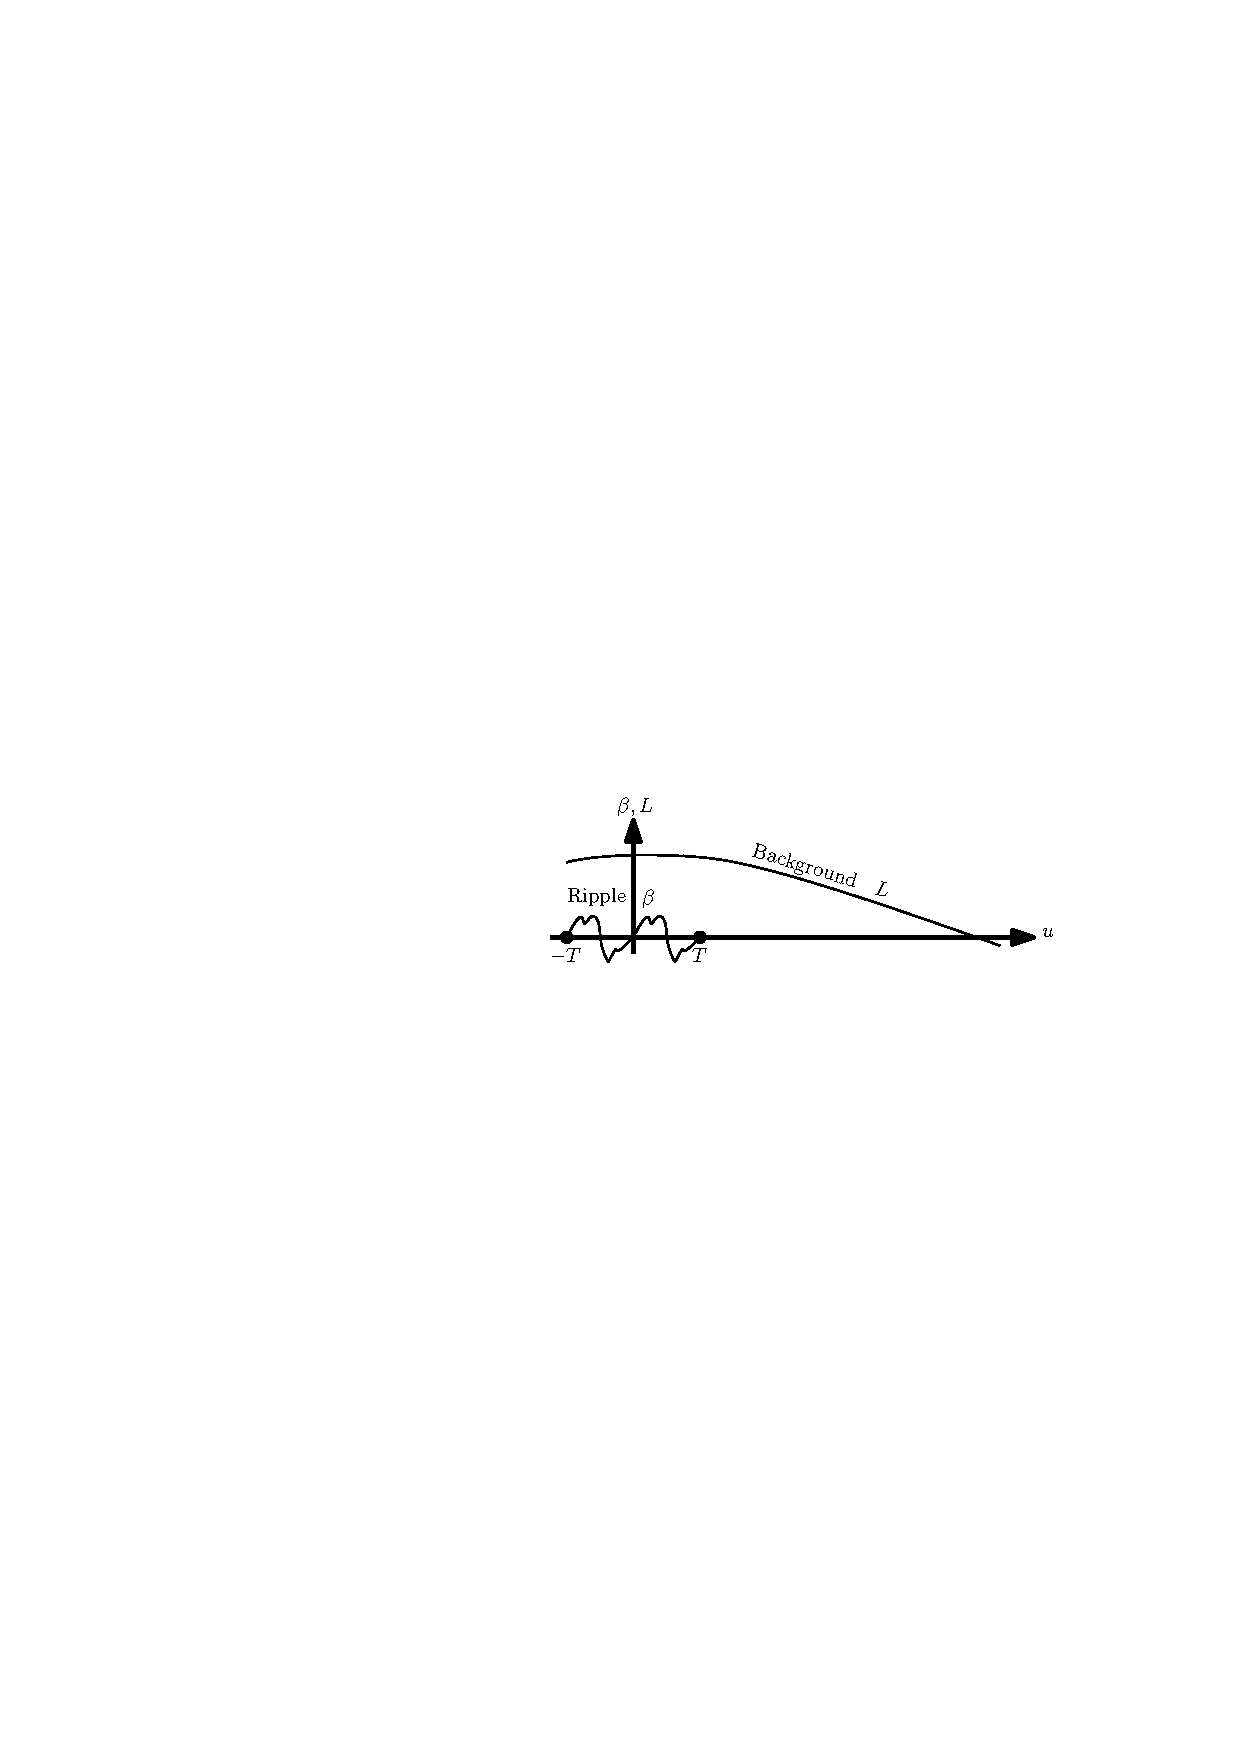
\includegraphics{Kap3/background.pdf}\caption{Pulse profile for an exact plane wave solution to Einstein field equations. Traced figure from \cite{GRAVITATION}.
\label{fig:pulse}}
\par\end{centering}
\end{figure}

We are going to take the case where $\beta\left(u\right)$ is a pulse
of duration $2T$, see figure \ref{fig:pulse}, and $\left|\beta'\right|\ll1/T$
throughout the pulse. We are going to take three cases:
\begin{itemize}
\item For $u<-T$, we have a flat spacetime, then the pulse has not yet
arrived. This means that
\[
\beta=0,\ L=1
\]
\item For $-T<u<T$, here we are in the interior of the pulse. In this case
we solve equation (\ref{eq:LL}) and we use this solution recursively
in such a way that
\begin{align*}
\beta & =\beta\left(u\right)\text{ is arbitrary, except that }\left|\beta'\right|\ll1/T\\
L\left(u\right) & =1-\int_{-T}^{u}\left\{ \int_{-T}^{\bar{u}}\left[\beta'\left(\bar{\bar{u}}\right)\right]^{2}d\bar{\bar{u}}\right\} d\bar{u}+\mathcal{O}\left(\left[b'T\right]^{4}\right)
\end{align*}
\item For $u>T$, here the pulse has passed, then
\[
\beta=0,\ L=1-\frac{u}{a},\ \text{where }a\equiv\frac{1+\mathcal{O}\left(\left[b'T\right]^{2}\right)}{\int_{-T}^{T}\left(\beta'\right)^{2}du}
\]
\end{itemize}
From equations (\ref{eq:rvxux}) and (\ref{eq:rvyuy}) we have that
these components vanish in any extended region where $\beta=0$. Thus
spacetime is completely flat in regions where the wave factor vanishes,
which is outside the pulse. In particular, spacetime is flat near
$u=a$, then here we have a coordinate singularity.

Let us consider now the line element
\[
ds^{2}=L^{2}\left(u\right)\left(dx^{2}+dy^{2}\right)-dudv
\]
which is always flat if satisfies the vacuum Einstein equations. In
this metric the electromagnetic potential
\[
\boldsymbol{A}=A_{\alpha}dx^{\alpha}=A\left(u\right)dx
\]
satisfies Maxwell's equations for an arbitrary $A\left(u\right)$.
The only nonzero field components of this wave are
\[
F_{ux}=A'
\]
or
\[
F_{tx}=-F_{zx}=A',
\]
then the electric vector oscillates back and forth in the $x$-direction,
the magnetic vector oscillates in the $y$-direction. To calculate
the momentum-energy tensor we use the following equation\footnote{For a simpler comparison we are going to set the constant values $c=G=1$,
but later we are going to return to the values of $c$ and $G$ in
the SI system.}
\[
T^{\alpha\beta}=\frac{1}{4\pi}\left[F^{\alpha\mu}F_{\mu}^{\beta}-\frac{1}{4}\eta^{\alpha\beta}F_{\mu\nu}F^{\mu\nu}\right],
\]
therefore in $x$, $y$, $u$, $v$ coordinates the non-vanishing
component of the momentum-energy tensor is
\[
T_{uu}=\left(\frac{1}{4\pi L^{2}}\right)\left(A'\right)^{2},
\]

The Maxwell equations are satisfied by the potential $A$ in the background
metric. We impose the Einstein equations $G_{\alpha\beta}=8\pi T_{\alpha\beta}$,
because always satisfies the vacuum Einstein equations the Einstein
tensor is equal to the Ricci tensor. Because we imposed the Einstein
equations then
\[
R_{uu}=8\pi\left(\frac{1}{4\pi L^{2}}\right)\left(A'\right)^{2},
\]
therefore in the vacuum
\[
L''+\left(4\pi T_{uu}\right)L=0
\]
which has exactly the form of the equation (\ref{eq:LL}), then the
electromagnetic plane wave and the gravitational plane wave produce
the same gravitational attractions, 
\[
\left[\frac{\left(\beta'\right)^{2}}{4\pi}\right]_{\text{Grav. Wave}}=\left[T_{uu}\right]_{\text{EM Wave}}=\frac{\left(A'\right)^{2}}{4\pi L^{2}}.
\]

We are going to hold the quantities $\left(\beta'\right)^{2}/4\pi$
and $\left(A'\right)^{2}/4\pi L^{2}$
\[
\left\langle \frac{\left(\beta'\right)^{2}}{4\pi}\right\rangle =\left\langle \frac{\left(A'\right)^{2}}{4\pi L^{2}}\right\rangle =\text{const.}
\]
with respect to this quantity we said that the reduce wavelength $\bar{\lambda}$
is small. With this is mind we are able to define the characteristic
length of the background geometry, radius of curvature of background
geometry, as 
\[
L_{b}\sim\left|\frac{L}{L''}\right|_{\begin{array}{l}
\text{Inside}\\
\text{the wave}
\end{array}}^{1/2}\sim\frac{1}{\left|\beta'\right|},
\]
from this we see that when there is no wave we return to the flat
spacetime.

\subsubsection*{Scale contribution of linearized gravitational field}

In a more general way, we find some coordinate system where we can
write the metric tensor just like in (\ref{eq:ggh}), the term $\overline{g}_{\alpha\beta}$
has a typical scale of spatial variation $L_{b}$, on top of which
small amplitude perturbations are superimposed, characterized by a
reduced wavelength $\bar{\lambda}$ such that
\begin{equation}
\bar{\lambda}\ll L_{b}.\label{ll}
\end{equation}
Then $h_{\alpha\beta}$ are, from a physical viewpoint, small ripples
on a smooth background. This can be done also in the frequency space,
if $\overline{g}_{\alpha\beta}$ has frequencies up to maximum value
$f_{b}$, while $h_{\alpha\beta}$ is peaked around a frequency $f$
such that
\begin{equation}
f\gg f_{b}.\label{ff}
\end{equation}
In this case $h_{\alpha\beta}$ is a high-frequency perturbation of
a static or slowly varying background. The scales $L_{b}$ and $f_{b}$
that characterize the background are unrelated, therefore we only
need that one of (\ref{ll}) and (\ref{ff}) be satisfied.

Now we are going to see from the typical variation scales how the
curvature is determined by gravitational waves and by matter\footnote{Here we return to the usual values of $c$ and $G$ in the SI system}.
First let us consider and expansion of the Ricci tensor to quadratic
order in $h_{\alpha\beta}$\footnote{For an extensive work of series expansion applied to tensors see HORTUA},
\begin{equation}
R_{\alpha\beta}=\bar{R}_{\alpha\beta}+R_{\alpha\beta}^{(1)}+R_{\alpha\beta}^{(2)}+\cdots,\label{eq:rr}
\end{equation}
where $\bar{R}_{\alpha\beta}$ is constructed with $\overline{g}_{\alpha\beta}$
only, $R_{\alpha\beta}^{(1)}$ is linear in $h_{\alpha\beta}$, $R_{\alpha\beta}^{(2)}$
is quadratic in $h_{\alpha\beta}$ and so on. We can calculate the
expressions of $R_{\alpha\beta}^{(1)}$ and $R_{\alpha\beta}^{(2)}$
in terms of $h_{\alpha\beta}$, $\overline{g}_{\alpha\beta}$ and
$\bar{\nabla}$, the covariant derivative with respect to the background\footnote{For details see MAGGIORE}
\begin{align}
R_{\alpha\beta}^{(1)}= & \ \frac{1}{2}\left(\bar{\nabla}^{\mu}\bar{\nabla}_{\alpha}h_{\beta\mu}+\bar{\nabla}^{\mu}\bar{\nabla}_{\beta}h_{\alpha\mu}-\bar{\nabla}^{\mu}\bar{\nabla}_{\mu}h_{\alpha\beta}-\bar{\nabla}_{\beta}\bar{\nabla}_{\alpha}h\right)\label{eq:r1h}\\
R_{\alpha\beta}^{(2)}= & \ \frac{1}{2}\overline{g}^{\rho\sigma}\overline{g}^{\mu\nu}\left[\frac{1}{2}\bar{\nabla}_{\alpha}h_{\rho\mu}\bar{\nabla}_{\beta}h_{\sigma\nu}+\left(\bar{\nabla}_{\rho}h_{\beta\mu}\right)\left(\bar{\nabla}_{\sigma}h_{\alpha\nu}-\bar{\nabla}_{\nu}h_{\alpha\sigma}\right)\right.\nonumber \\
\  & \ h_{\rho\mu}\left(\bar{\nabla}_{\beta}\bar{\nabla}_{\alpha}h_{\sigma\nu}+\bar{\nabla}_{\nu}\bar{\nabla}_{\sigma}h_{\alpha\beta}-\bar{\nabla}_{\nu}\bar{\nabla}_{\beta}h_{\alpha\sigma}-\bar{\nabla}_{\nu}\bar{\nabla}_{\alpha}h_{\beta\sigma}\right)\nonumber \\
\  & \ \left(\frac{1}{2}\bar{\nabla}_{\mu}h_{\rho\sigma}-\bar{\nabla}_{\rho}h_{\mu\sigma}\right)\left(\bar{\nabla}_{\beta}h_{\alpha\nu}+\bar{\nabla}_{\alpha}h_{\beta\nu}-\bar{\nabla}_{\nu}h_{\alpha\beta}\right)\label{eq:r2h}
\end{align}
 and with this one finds that the order of magnitude of $\bar{R}_{\alpha\beta}$
in the absence of matter fields reads
\[
\bar{R}_{\alpha\beta}\sim\left(\partial h\right)^{2},
\]
this means that the derivatives of $h_{\alpha\beta}$ affect the curvature
of the background metric $\overline{g}_{\alpha\beta}$. The scale
of variation of $\overline{g}_{\alpha\beta}$ is $L_{b}$ and of $h_{\alpha\beta}$
is $\bar{\lambda}$, then
\[
\partial\overline{g}_{\alpha\beta}\sim\frac{(\text{typical value of }\overline{g}_{\alpha\beta})}{L_{b}},
\]
while
\begin{equation}
\partial h\sim\frac{(\text{typical value of }h_{\alpha\beta})}{\bar{\lambda}}.\label{eq:dh}
\end{equation}
The background expression $\bar{R}_{\alpha\beta}$ is constructed
from the second derivatives of the background metric, then, if we
set the typical values of $\overline{g}_{\alpha\beta}$ to one rescaling
our coordinates
\[
\bar{R}_{\alpha\beta}\sim\partial^{2}\overline{g}_{\alpha\beta}\sim\frac{1}{L_{b}^{2}},
\]
while from (\ref{eq:dh})
\[
\left(\partial h\right)^{2}\sim\left(\frac{h}{\bar{\lambda}}\right)^{2},
\]
therefore we have the relation
\[
\frac{1}{L_{b}^{2}}\sim\left(\frac{h}{\bar{\lambda}}\right)^{2},
\]
that is
\[
h\sim\frac{\bar{\lambda}}{L_{b}},
\]
which is the curvature determined by gravitational radiation. If we
consider a non-vanishing energy-momentum tensor, the contribution
of gravitational waves to the background curvature is negligible compared
to the contribution of matter sources. Then the background curvature
will be much bigger than the contribution of gravitational waves,
\[
h\ll\frac{\bar{\lambda}}{L_{b}}.
\]

\subsubsection{How gravitational waves in linearized gravity curve the background}

We take a coordinate system in which we can split the metric tensor,
in a metric background and the linearized gravitational field. We
can split the metric in this way because we have a clear distinction
of scales, then one of the conditions, (\ref{ll}) or (\ref{ff}),
applies. From the Einstein equations written in the form
\[
R_{\alpha\beta}=\frac{8\pi G}{c^{4}}\left(T_{\alpha\beta}-\frac{1}{2}g_{\alpha\beta}T\right),
\]
where $T$ is the trace of the energy-momentum tensor $T_{\alpha\beta}$.
We take again the expansion of the Ricci tensor like is shown in the
expression (\ref{eq:rr}). We know the differences of frequencies
between gravitational waves and background, then this allows to split
the Einsteins field equations into two separate parts, the low and
the high frequency parts, 
\begin{align}
\bar{R}_{\alpha\beta}= & \ -\left[R_{\alpha\beta}^{(2)}\right]^{\text{Low}}+\frac{8\pi G}{c^{4}}\left(T_{\alpha\beta}-\frac{1}{2}g_{\alpha\beta}T\right)_{,}^{\text{Low}}\label{eq:rlow}\\
R_{\alpha\beta}^{(1)}= & \ -\left[R_{\alpha\beta}^{(2)}\right]^{\text{High}}+\frac{8\pi G}{c^{4}}\left(T_{\alpha\beta}-\frac{1}{2}g_{\alpha\beta}T\right)_{,}^{\text{High}}\label{eq:rhigh}
\end{align}
where ``Low'' denotes the projection on the low frequencies and
``High'' for the high ones. We can also work with the length scales
if we want to.

\subsubsection*{Computation of averages}

Given that the gravitational energy can not be located, an average
is made over the tensor fields. Integrating a tensor field does not
give a tensor in a curved space, because tensors at different points
have different transformation properties. To be able to sum tensors
in different points we must transport in parallel to add in a common
point.

Let us introduce the bivector of geodesic parallel displacement,
denoted by $\gamma_{\alpha}^{\beta'}\left(\boldsymbol{x},\boldsymbol{x}'\right)$.
This transforms as a vector with respect to coordinate transformations
at either $\boldsymbol{x}$ or $\boldsymbol{x}'$, and, assuming that
$\boldsymbol{x}$ and $\boldsymbol{x}'$ are sufficiently close together
to insure the existence of a unique geodesic of the metric $\bar{g}_{\alpha\beta}$,
where $\bar{g}_{\alpha\beta}$ is the background geometry, between
them, given the vector components $A_{\alpha'}$ at $\boldsymbol{x}'$,
then $A_{\alpha}=\gamma_{\alpha}^{\alpha'}A_{\alpha'}$ is the unique
vector at x which can be obtained by transporting in parallel $A_{\alpha'}$
from $\boldsymbol{x}'$ back to $\boldsymbol{x}$ along the geodesic.

Let $T_{\alpha\beta}$ be a tensor and let us assume that have high
frequency components of wavelength $\lambda$ and a background geometry
$\bar{g}_{\alpha\beta}$ containing only low frequency components
of wavelength $L\gg\lambda$, then we define the average of $T_{\alpha\beta}$
to be the tensor
\[
\left\langle T_{\alpha\beta}\left(\boldsymbol{x}\right)\right\rangle =\int_{\text{all space}}g_{\alpha}^{\alpha'}\left(\boldsymbol{x},\boldsymbol{x}'\right)g_{\beta}\left(\boldsymbol{x},\boldsymbol{x}'\right)T_{\alpha'\beta'}\left(\boldsymbol{x}'\right)f\left(\boldsymbol{x},\boldsymbol{x}'\right)d^{4}x'
\]
where $f\left(\boldsymbol{x},\boldsymbol{x}'\right)$ is a weighting
function which falls smoothly to zero when $\boldsymbol{x}$ and $\boldsymbol{x}'$
differ by a distance $d$ such that $\bar{\lambda}\ll d\ll L$ and
\[
\int_{\text{all space}}f\left(\boldsymbol{x},\boldsymbol{x}'\right)d^{4}x'=1
\]

What we are doing here, in a more physical way, is to average over
several wavelengths if (\ref{ll}) applies, or a temporal average
over several periods of the gravitational waves if (\ref{ff}) applies.
An advantage of this average is that the derivatives will average
to zero,
\[
\left\langle \partial_{\mu}A\right\rangle =0,
\]
then
\[
\left\langle A\left(\partial_{\mu}B\right)\right\rangle =-\left\langle \left(\partial_{\mu}A\right)B\right\rangle .
\]

With this in mind, we write equation (\ref{eq:rlow}) as
\begin{equation}
\bar{R}_{\alpha\beta}=-\left\langle R_{\alpha\beta}^{(2)}\right\rangle +\frac{8\pi G}{c^{4}}\left\langle T_{\alpha\beta}-\frac{1}{2}g_{\alpha\beta}T\right\rangle ,\label{eq:rprom}
\end{equation}
let us define the tensor $t_{\alpha\beta}$ such that
\[
-\left\langle R_{\alpha\beta}^{(2)}\right\rangle =\frac{8\pi G}{c^{4}}\left(t_{\alpha\beta}-\frac{1}{2}\bar{g}_{\alpha\beta}t\right),
\]
where $t=\bar{g}^{\alpha\beta}t_{\alpha\beta}$. Because $\bar{g}_{\alpha\beta}$
is a pure low-frequency quantity then $\left\langle \bar{g}^{\alpha\beta}R_{\alpha\beta}^{(2)}\right\rangle =\bar{g}^{\alpha\beta}\left\langle R_{\alpha\beta}^{(2)}\right\rangle $
and $\bar{g}^{\alpha\beta}\bar{g}_{\alpha\beta}=4$, this allow us
to find an expression for $t_{\alpha\beta}$
\begin{equation}
t_{\alpha\beta}=-\frac{c^{4}}{8\pi G}\left\langle R_{\alpha\beta}^{(2)}-\frac{1}{2}\bar{g}_{\alpha\beta}R^{(2)}\right\rangle \label{emtensor}
\end{equation}
where $R^{(2)}=\bar{g}^{\alpha\beta}R_{\alpha\beta}^{(2)}$, the equation
(\ref{emtensor}) is the energy-momentum tensor of gravitational waves
in linearized gravity. We can rewrite equations (\ref{eq:rprom}) as
\[
\bar{R}_{\alpha\beta}=\frac{8\pi G}{c^{4}}\left(t_{\alpha\beta}-\frac{1}{2}\bar{g}_{\alpha\beta}t\right)+\frac{8\pi G}{c^{4}}\left(T_{\alpha\beta}-\frac{1}{2}g_{\alpha\beta}T\right),
\]
or in an equivalent way
\[
\bar{R}_{\alpha\beta}-\frac{1}{2}\bar{g}_{\alpha\beta}\bar{R}=\frac{8\pi G}{c^{4}}\left(\bar{T}_{\alpha\beta}+t_{\alpha\beta}\right).
\]
Due to the Bianchi identity we have
\[
\bar{\nabla}^{\beta}\left(T_{\beta\alpha}+t_{\beta\alpha}\right)=0,
\]
and if $T_{\beta\alpha}=0$ then
\begin{equation}
\bar{\nabla}^{\beta}t_{\beta\alpha}=0.\label{eq:tbianchi}
\end{equation}

\subsubsection{The energy-momentum tensor of gravitational waves and the flux of
energy and momentum\label{sec:energy}}

In above section we obtain an expression for the energy-momentum
tensor of gravitational waves in linearized gravity, equation (\ref{emtensor}).
Now we are going to return to the flat background metric splitting,
equation (\ref{gl}), then in our equations (\ref{eq:r1h}) and (\ref{eq:r2h})
we replace $\bar{\nabla}_{\alpha}\rightarrow\partial_{\alpha}$. Applying
the DeDonder gauge (\ref{hg}) and the TT gauge (\ref{gtt}), the
equation (\ref{eq:r2h}) is written as follows
\[
\left\langle R_{\alpha\beta}^{(2)}\right\rangle =-\frac{1}{4}\left\langle \partial_{\alpha}h_{\mu\nu}\partial_{\beta}h^{\mu\nu}\right\rangle ,
\]
therefore the equation (\ref{emtensor}) is now
\[
t_{\alpha\beta}=\frac{c^{4}}{32\pi G}\left\langle \partial_{\alpha}h_{\mu\nu}\partial_{\beta}h^{\mu\nu}\right\rangle .
\]
In particular the $t_{00}$ component is then
\[
t^{00}=\frac{c^{2}}{32\pi G}\left\langle \dot{h}_{ij}^{TT}\dot{h}_{ij}^{TT}\right\rangle ,
\]
if we assume again the direction of the gravitational wave, just like
in (\ref{eq:kz}), we can write $t_{00}$ in terms of $h_{+}$ and
$h_{\times}$,
\[
t^{00}=\frac{c^{2}}{16\pi G}\left\langle \dot{h}_{+}^{2}+\dot{h}_{\times}^{2}\right\rangle .
\]

Now we want to obtain an expression for the radiated power of the
gravitational radiation. The gravitational wave energy inside the
volume $V$ is\footnote{see Chapter 3 to check the expression of energy and momentum}
\[
E_{V}=\int_{V}t^{00}d^{3}x,
\]
from equation (\ref{eq:tbianchi})
\[
\int_{V}\left(\partial_{0}t^{00}+\partial_{i}t^{i0}\right)d^{3}x=0,
\]
we have
\[
\frac{1}{c}\frac{dE_{v}}{dt}=-\int_{V}\partial_{i}t^{i0}d^{3}x=-\int_{S}n_{i}t^{0i}dA
\]
where $n^{i}$ is the outer normal to the surface $S$ and $dA$ is
the surface element. Taking its normal in the unitary radial direction
\begin{align*}
\frac{dE_{v}}{dt}= & \ -c\int_{S}t^{0r}dA,\\
t^{0r}= & \ \frac{c^{2}}{32\pi G}\left\langle \partial^{0}h_{ij}^{TT}\partial_{r}h_{ij}^{TT}\right\rangle .
\end{align*}
At sufficiently large distances $r$, just like in electrodynamics,
the linearized gravitational field has the general form
\[
h_{ij}^{TT}\left(t,r\right)=\frac{1}{r}f_{ij}\left(t-\frac{r}{c}\right)
\]
then
\[
\partial_{r}h_{ij}^{TT}\left(t,r\right)=-\frac{1}{r^{2}}f_{ij}\left(t-\frac{r}{c}\right)+\frac{1}{r}\partial_{r}f_{ij}\left(t-\frac{r}{c}\right).
\]
On a function of the combination $t-r/c$ we have
\[
\partial_{r}f_{ij}\left(t-\frac{r}{c}\right)=-c^{-1}\partial_{t}f_{ij}\left(t-\frac{r}{c}\right),
\]
therefore
\begin{align*}
\partial_{r}h_{ij}^{TT}\left(t,r\right)= & \ -\partial_{0}h_{ij}^{TT}\left(t,r\right)+O\left(1/r^{2}\right),\\
= & \ \partial^{0}h_{ij}^{TT}\left(t,r\right)+O\left(1/r^{2}\right).
\end{align*}
From above equation, at large distances $t^{0r}=t^{00}$, therefore
the energy inside a volume $V$ satisfies
\[
\frac{dE_{v}}{dt}=-c\int_{S}t^{00}dA,
\]
the fact that $E_{V}$ decreases means that the outward-propagating
gravitational wave carries away an energy flux. Writing the surface
element $dA=r^{2}d\Omega$
\[
\frac{dE}{dt}=\frac{c^{3}r^{2}}{32\pi G}\int\left\langle \partial_{t}h_{ij}^{TT}\partial_{t}h_{ij}^{TT}\right\rangle d\Omega,
\]
in terms of $h^{+}$ and $h^{\times}$
\begin{equation}
\label{eq:dedt-ch2}
\frac{dE}{dt}=\frac{c^{3}r^{2}}{16\pi G}\int\left\langle \left(\partial_{t}h^{+}\right)^{2}+\left(\partial_{t}h^{\times}\right)^{2}\right\rangle d\Omega.
\end{equation}

In the same way we can compute the flux of momentum. The momentum
of the gravitational wave inside a spherical shell $V$ at large
distances from the source is
\[
P^{i}=\frac{1}{c}\int_{V}t^{0i}dx^{3},
\]
we consider, again, a propagating radially outward gravitational wave,
in a similar way that we did with the energy flux
\begin{align*}
c\partial_{0}P^{i}= & \ \int_{V}\partial_{0}t^{0i}d^{3}x\\
= & \ -\int t^{0i}dA,
\end{align*}
therefore the momentum flux carried away by the gravitational wave
along the radial direction is
\[
\frac{dP^{k}}{dt}=-\frac{c^{3}r^{2}}{32\pi G}\int\left\langle \partial_{t}h_{ij}^{TT}\partial^{k}h_{ij}^{TT}\right\rangle d\Omega.
\]

\subsection{Quadrupolar contribution of linearized gravity}

In section 1 was discussed the dipolar contribution of radiation in
electrodynamics. Here we will see from which contribution starts to
radiate. It is a fact given the positive value nature of masses is
not able to produce a dipole oscillating system just like in electrodynamics,
then we can expect that the main contribution of radiation is the
quadrupolar contribution. The idea is to see in an analytical way
that we have such contribution.

Let us assume an isolated source that is far away from an observer
and is slowly moving, this means that most of the radiation emitted
will be at frequencies $\omega$ sufficiently low that if $d$ is
the source size then $d\ll\omega^{-1}$, or $d\ll\bar{\lambda}$.
To perform the multipole expansion we start from the expression
\[
h_{ij}^{TT}=\frac{1}{r}\frac{4G}{c^{4}}\Lambda_{ij,kl}\left(\hat{\boldsymbol{n}}\right)\int T_{kl}\left(t-\frac{r}{c}+\frac{\boldsymbol{x}'\cdot\hat{\boldsymbol{n}}}{c},\boldsymbol{x}'\right)d^{3}x'
\]
we write $T_{kl}$ in terms of its Fourier transformation
\begin{equation}
T_{kl}\left(t-\frac{r}{c}+\frac{\boldsymbol{x}'\cdot\hat{\boldsymbol{n}}}{c},\boldsymbol{x}'\right)=\frac{1}{\left(2\pi\right)^{4}}\int\widetilde{T}_{kl}\left(\omega,\boldsymbol{k}\right)e^{-i\omega\left(t-r/c+\boldsymbol{x}'\cdot\hat{\boldsymbol{n}}/c\right)+i\boldsymbol{k}\cdot\boldsymbol{x}'}d^{4}k\label{eq:fourier}
\end{equation}
given the radiation conditions, $\widetilde{T}_{kl}\left(\omega,\boldsymbol{k}\right)$
is peaked around a typical frequency $\omega$ with $\omega d\ll c$.
On the other hand, the energy momentum tensor is non-vanishing only
inside the source, so we restrict ourselves to $\left|\boldsymbol{x}'\right|\leq d$.
Then the dominant contribution to $h_{ij}^{TT}$ comes from frequencies
$\omega$ that satisfy
\[
\frac{\omega}{c}\boldsymbol{x}'\cdot\boldsymbol{n}\apprle\frac{\omega d}{c}\ll 1,
\]
and therefore we can expand the exponential in equation (\ref{eq:fourier})
\[
e^{-i\omega\left(t-r/c+\boldsymbol{x}'\cdot\hat{\boldsymbol{n}}/c\right)+i\boldsymbol{k}\cdot\boldsymbol{x}'}=e^{-i\omega\left(t-r/c\right)}\left[1-i\frac{\omega}{c}{x'}^{i}n^{i}+\frac{1}{2}\left(-i\frac{\omega}{c}\right)^{2}{x'}^{i}{x'}^{j}n^{i}n^{j}+\cdots\right],
\]
therefore
\[
T_{kl}\left(t-\frac{r}{c}+\frac{\boldsymbol{x}'\cdot\hat{\boldsymbol{n}}}{c},\boldsymbol{x}'\right)\approx T_{kl}\left(t-\frac{r}{c},\boldsymbol{x}'\right)+\frac{{x'}^{i}n^{i}}{c}\partial_{0}T_{kl}+\frac{1}{2c^{2}}{x'}^{i}{x'}^{j}n^{i}n^{j}\partial_{0}^{2}T_{kl}+\cdots
\]
where all derivatives are evaluated at the point $\left(t-r/c,\boldsymbol{x}'\right)$.
Let us define the momenta stress tensor of $T^{ij}$ as

\begin{align*}
S^{ij} & =\int T^{ij}\left(t,\boldsymbol{x}\right)d^{3}x\\
S^{ij,k} & =\int T^{ij}\left(t,\boldsymbol{x}\right)x^{k}d^{3}x\\
S^{ij,kl} & =\int T^{ij}\left(t,\boldsymbol{x}\right)x^{k}x^{l}d^{3}x\\
\  & \ \ \ \ \ \ \vdots
\end{align*}
where the comma separates the spatial indices, which originates from
$T^{ij}$, from the indices coming from $x^{i}$. Given the symmetry
of $T^{ij}$, then $S^{ij,k}=S^{ji,k}$, but not necessarily is symmetric
under the change of indices of different type, $S^{ij,k}\neq S^{ik,j}$.

\begin{align}
h_{ij}^{TT} & =\frac{1}{r}\frac{4G}{c^{4}}\Lambda_{ij,kl}\left(\hat{\boldsymbol{n}}\right)\int T_{kl}\left(t-\frac{r}{c}+\frac{\boldsymbol{x}'\cdot\hat{\boldsymbol{n}}}{c},\boldsymbol{x}'\right)d^{3}x'\\
\  & \approx\frac{1}{r}\frac{4G}{c^{4}}\Lambda_{ij,kl}\left(\hat{\boldsymbol{n}}\right)\left[\int T^{kl}d^{3}x'+\frac{1}{c}n_{m}\partial_{t}\int T^{kl}{x'}^{m}d^{3}x'+\frac{1}{2c^{2}}n_{m}n_{p}\partial_{t}\partial_{t}\int T^{kl}{x'}^{m}{x'}^{p}d^{3}x'+\cdots\right]_{\text{ret}}\\
\  & =\frac{1}{r}\frac{4G}{c^{4}}\Lambda_{ij,kl}\left(\hat{\boldsymbol{n}}\right)\left[S^{kl}+\frac{1}{c}n_{m}\partial_{t}S^{kl,m}+\frac{1}{2c^{2}}n_{m}n_{p}\partial_{t}\partial_{t}S^{kl,mp}+\cdots\right]_{\text{ret}},\label{eq:h-exp-s}
\end{align}
where the subscript ``ret'' means that the quantities $S^{kl}$,
$S^{kl,m}$, $S^{kl,ml}$, etc. are evaluated at the retarded time.
Let us define the mass density as\footnote{This is a consequence of the expression of energy}
\begin{align*}
M & =\frac{1}{c^{2}}\int T^{00}\left(t,\boldsymbol{x}\right)d^{3}x\\
M^{i} & =\frac{1}{c^{2}}\int T^{00}\left(t,\boldsymbol{x}\right)x^{i}d^{3}x\\
M^{ij} & =\frac{1}{c^{2}}\int T^{00}\left(t,\boldsymbol{x}\right)x^{i}x^{j}d^{3}x\\
M^{ijk} & =\frac{1}{c^{2}}\int T^{00}\left(t,\boldsymbol{x}\right)x^{i}x^{j}x^{k}d^{3}x\\
\  & \ \ \ \ \ \ \vdots
\end{align*}
while the momentum density is given by\footnote{Just like it was mention before, the obtaining of this expression is
obtained forward}
\begin{align*}
P^{i} & =\frac{1}{c}\int T^{0i}\left(t,\boldsymbol{x}\right)d^{3}x\\
P^{i,j} & =\frac{1}{c}\int T^{0i}\left(t,\boldsymbol{x}\right)x^{j}d^{3}x\\
P^{i,jk} & =\frac{1}{c}\int T^{0i}\left(t,\boldsymbol{x}\right)x^{j}x^{k}d^{3}x.\\
\  & \ \ \ \ \ \ \vdots
\end{align*}

We are going to obtain identities to obtain the quadrupolar contribution.
Given that $\partial_{\beta}T^{\alpha\beta}=0$
\[
\partial_{0}T^{00}=-\partial_{i}T^{0i}
\]
we integrate in the hole space
\[
c\partial_{t}M=\int\partial_{0}T^{00}d^{3}x=-\int T^{0i}dS^{i}=-\int T^{0i}dS^{i}=0,
\]
this means that we are taking the boundary where there is no matter
field, then in this boundary $T^{0i}$ vanishes. In a similar way
\begin{align*}
c\partial_{t}M^{i} & =\int\partial_{0}T^{00}x^{i}d^{3}x=-\int\partial_{j}T^{0j}x^{i}d^{3}x=\int T^{0j}\partial_{j}x^{i}d^{3}x=\int T^{0j}\delta_{j}^{i}d^{3}x\\
\  & =\int T^{0i}d^{3}x=cP^{i},
\end{align*}
this process can be done for the higher order momentum, therefore
\begin{align}
\partial_{t}M & =0\\
\partial_{t}M^{i} & =P^{i}\\
\partial_{t}M^{ij} & =P^{i,j}+P^{j,i}\label{eq:dmdtp}\\
\partial_{t}M^{ijk} & =P^{i,jk}+P^{j,ki}+P^{k,ij}
\end{align}
now for the case of the stress
\[
c\partial_{t}P^{i}=\int\partial_{0}T^{0i}d^{3}x=-\int T^{ji}dS^{j}=0
\]
just like the mass density, and
\begin{align*}
c\partial_{t}P^{i,j} & =\int\partial_{0}T^{0i}x^{j}d^{3}x=-\int\partial_{k}T^{ki}x^{j}d^{3}x=\int T^{ki}\partial_{k}x^{j}d^{3}x=\int T^{ki}\delta_{k}^{j}d^{3}x\\
\  & =\int T^{ij}d^{3}x=S^{ij},
\end{align*}
therefore
\begin{align}
\partial_{t}P^{i} & =0\\
\partial_{t}P^{i,j} & =S^{ij}\label{eq:dpdts}\\
\partial_{t}P^{i,jk} & =S^{ij,k}+S^{ik,j}.
\end{align}
The equations $\partial_{t}M=0$ and $\partial_{t}P^{i}=0$ are the
conservation of the mass and the conservation of the total momentum
of the source. Derivating (\ref{eq:dmdtp}) with respect $t$, using
(\ref{eq:dpdts}) and the fact that $S^{ij}=S^{ji}$ then
\begin{equation}
S^{ij}=\frac{1}{2}\ddot{M}^{ij}.\label{eq:sm}
\end{equation}

We are going to use (ref{eq:sm}) as the leading term in the expansion
(\ref{eq:h-exp-s}),
\[
h_{ij}^{TT}\left(t,\boldsymbol{x}\right)\approx\frac{1}{r}\frac{2G}{c^{4}}\Lambda_{ij,kl}\left(\hat{\boldsymbol{n}}\right)\ddot{M}_{ij},
\]
we decompose $\ddot{M}^{ij}$ in the following way
\begin{equation}
\ddot{M}^{ij}=\left(\ddot{M}^{ij}-\frac{1}{3}\delta^{ij}M_{kk}\right)+\frac{1}{3}\delta^{ij}M_{kk},\label{eq:mij-tr}
\end{equation}
where $M_{kk}$ is the trace of $M_{ij}$. Because $\Lambda_{ij,kl}\delta^{kl}=\Lambda_{ij,kk}=0$,
we have contribution only from the traceless term of (\ref{eq:mij-tr}),
let us denote this term as follows
\[
Q^{ij}=\ddot{M}^{ij}-\frac{1}{3}\delta^{ij}M_{kk},
\]
therefore
\begin{align*}
h_{ij}^{TT}\left(t,\boldsymbol{x}\right) & \approx\frac{1}{r}\frac{2G}{c^{4}}\Lambda_{ij,kl}\left(\hat{\boldsymbol{n}}\right)Q_{ij}\left(t-\frac{r}{c}\right)\\
\  & =\frac{1}{r}\frac{2G}{c^{4}}Q_{ij}^{TT}\left(t-\frac{r}{c}\right)
\end{align*}
which is the quadrupolar contribution.
